%% ============================================================
%%  OFDM Based Wireless Communication System
%%  Graduation Project Report
%%  Ankara Yıldırım Beyazıt University
%%  Department of Electrical and Electronics Engineering
%%  Student: Kemal Sercan İlhan  |  222050211002
%% ============================================================
\documentclass[12pt, a4paper, oneside]{report}

%% ---- Encoding & Language -----------------------------------
\usepackage[utf8]{inputenc}
\usepackage[T1]{fontenc}
\usepackage[english]{babel}

%% ---- Page Layout ------------------------------------------
\usepackage[top=3cm, bottom=2.5cm, left=3.5cm, right=2.5cm]{geometry}

%% ---- Typography -------------------------------------------
\usepackage{times}          % Times New Roman-equivalent
\usepackage{setspace}
\onehalfspacing             % 1.5-line spacing (AYBU standard)

%% ---- Headers / Footers ------------------------------------
\usepackage{fancyhdr}
\pagestyle{fancy}
\fancyhf{}
\fancyhead[R]{\small\nouppercase{\leftmark}}
\fancyfoot[C]{\thepage}
\renewcommand{\headrulewidth}{0.4pt}

%% ---- Figures & Tables -------------------------------------
\usepackage{graphicx}
\usepackage{float}
\usepackage{caption}
\usepackage{subcaption}
\usepackage{booktabs}
\usepackage{array}
\usepackage{longtable}
\captionsetup{font=small, labelfont=bf, justification=centering}

%% ---- Math -------------------------------------------------
\usepackage{amsmath}
\usepackage{amssymb}

%% ---- Source Code Listing ----------------------------------
\usepackage{listings}
\usepackage{xcolor}
\lstdefinestyle{cstyle}{
  basicstyle=\ttfamily\footnotesize,
  keywordstyle=\color{blue}\bfseries,
  commentstyle=\color{gray},
  stringstyle=\color{red!70!black},
  breaklines=true,
  frame=single,
  numbers=left,
  numberstyle=\tiny\color{gray},
  tabsize=4,
}
\lstset{style=cstyle}

%% ---- Hyperlinks -------------------------------------------
\usepackage[hidelinks]{hyperref}
\usepackage{url}

%% ---- Misc -------------------------------------------------
\usepackage{parskip}        % space between paragraphs instead of indent
\usepackage{enumitem}
\usepackage{multirow}
\usepackage{pdfpages}

%% ---- Chapter title formatting (AYBU style) ----------------
\usepackage{titlesec}
\titleformat{\chapter}[block]
  {\normalfont\large\bfseries\centering}{CHAPTER \thechapter}{1em}{\MakeUppercase}
\titlespacing*{\chapter}{0pt}{0pt}{20pt}

\titleformat{\section}
  {\normalfont\normalsize\bfseries}{\thesection}{1em}{}
\titleformat{\subsection}
  {\normalfont\normalsize\bfseries\itshape}{\thesubsection}{1em}{}

%% ---- Placeholder helper -----------------------------------
\newcommand{\imgplaceholder}[2][6cm]{%
  \begin{figure}[H]
    \centering
    \fbox{\parbox[c][#1][c]{12cm}{\centering\small\textit{#2}}}
  \end{figure}%
}

%% ---- TikZ block-diagram support ---------------------------
\usepackage{tikz}
\usetikzlibrary{shapes.geometric,arrows.meta,positioning,fit,backgrounds,calc}
\tikzset{
  %% Generic filled rectangle block
  blk/.style 2 args={draw=black, fill=#1, text centered, rounded corners=3pt,
                     minimum height=0.88cm, font=\small, inner xsep=5pt,
                     inner ysep=4pt, text width=#2},
  blk/.default={blue!12}{2.4cm},
  %% Single-arg shorthand: blkc{color} – width stays default
  blkc/.style={blk={#1}{2.4cm}},
  %% Narrow variant
  nblk/.style={blk={#1}{1.7cm}},
  nblk/.default={blue!12},
  %% Wide variant
  wblk/.style={blk={#1}{3.2cm}},
  wblk/.default={blue!12},
  %% Flowchart terminal (rounded ends)
  term/.style={draw, fill=gray!20, rounded rectangle, text centered,
               minimum height=0.85cm, font=\small, inner sep=5pt},
  %% Decision diamond
  dec/.style={diamond, draw, fill=orange!20, text centered, aspect=2.4,
              font=\footnotesize, inner sep=2pt},
  %% Arrows
  arr/.style ={-{Stealth[length=3mm,width=2mm]}, thick},
  darr/.style={{Stealth[length=3mm,width=2mm]}-{Stealth[length=3mm,width=2mm]}, thick},
  sarr/.style={-{Stealth[length=2.5mm,width=1.8mm]}, semithick, dashed},
}

%% ============================================================
\begin{document}

%% ============================================================
%%  FRONT MATTER
%% ============================================================
\pagenumbering{roman}

%% ---- Cover Page -------------------------------------------
\begin{titlepage}
  \begin{center}
    \vspace*{0.5cm}
    {\Large\bfseries ANKARA YILDIRIM BEYAZIT UNIVERSITY}\\[0.4cm]
    {\large\bfseries GRADUATE SCHOOL OF NATURAL AND APPLIED SCIENCES}\\[0.2cm]
    {\large\bfseries DEPARTMENT OF ELECTRICAL AND ELECTRONICS ENGINEERING}\\[2.0cm]

    % Upload aybu_logo.png to Overleaf then replace the line below:
    % \includegraphics[width=4cm]{aybu_logo}
    \fbox{\parbox[c][4cm][c]{4cm}{\centering University Logo}}
    \\[2.0cm]

    {\LARGE\bfseries OFDM BASED WIRELESS COMMUNICATION SYSTEM}\\[1.5cm]

    {\large GRADUATION PROJECT}\\[2.0cm]

    {\large Kemal Sercan \textsc{İLHAN}}\\[0.2cm]
    {\normalsize Student No: 222050211002}\\[2.0cm]

    {\normalsize Supervisor: [Supervisor Name \& Title]}\\[2.5cm]

    {\normalsize Ankara, \the\year}
  \end{center}
\end{titlepage}

%% ---- Abstract ---------------------------------------------
\chapter*{ABSTRACT}
\addcontentsline{toc}{chapter}{Abstract}
\thispagestyle{plain}

\begin{center}
  {\large\bfseries OFDM Based Wireless Communication System}\\[0.5cm]
  Kemal Sercan İlhan\\
  Ankara Yıldırım Beyazıt University\\
  Department of Electrical and Electronics Engineering
\end{center}

\vspace{0.5cm}

This graduation project presents the design, implementation, and verification of an Orthogonal Frequency Division Multiplexing (OFDM) based wireless communication system using reconfigurable hardware. The system is built on a ZedBoard development platform equipped with a Xilinx Zynq-7020 System-on-Chip (SoC) and an Analog Devices FMCOMMS3 radio card hosting the AD9361 RF transceiver. The physical-layer waveform follows the IEEE 802.11a/n standard with 64 sub-carriers, a 312.5 kHz sub-carrier spacing, and a 20 MHz signal bandwidth.

The hardware description language (HDL) design integrates open-source OFDM transmitter and receiver IP cores with a custom AWGN channel emulation module, all synthesised in a Vivado block design targeting the Zynq programmable logic fabric. The ARM Cortex-A9 processing system is programmed with bare-metal C firmware built on the Analog Devices NO-OS framework, which handles RF parameter configuration, packet generation, and data acquisition. A Python-based graphical user interface (GUI) communicates with the embedded firmware over a serial link and provides real-time visualisation of bit-error-rate (BER), IQ constellations, time-domain waveforms, frequency-domain power spectra, and raw packet data.

The project demonstrates an end-to-end OFDM link in loopback and AWGN-emulated channel conditions, providing a practical platform for investigating digital communications concepts at the physical layer.

\vspace{0.5cm}
\noindent\textbf{Keywords:} OFDM, ZedBoard, Zynq-7020, AD9361, FPGA, NO-OS, SDR, BER, IEEE 802.11a, HDL, GNU Radio.

%% ---- Acknowledgements -------------------------------------
\chapter*{ACKNOWLEDGEMENTS}
\addcontentsline{toc}{chapter}{Acknowledgements}
\thispagestyle{plain}

I would like to express my sincere gratitude to my project supervisor for their continuous guidance, constructive feedback, and support throughout the course of this graduation project. Their expertise in digital communication systems and embedded hardware design has been invaluable in shaping the direction and quality of this work.

I am grateful to the faculty and staff of the Department of Electrical and Electronics Engineering at Ankara Yıldırım Beyazıt University for providing a stimulating academic environment and access to the necessary laboratory resources.

I also acknowledge the open-source hardware and software communities, particularly the contributors to the OpenOFDM project and the Analog Devices HDL and NO-OS repositories, whose work formed the technical foundation of this system.

Finally, I am deeply thankful to my family and friends for their patience, encouragement, and moral support during the demanding process of completing this project.

\vspace{1cm}
\begin{flushright}
Kemal Sercan İlhan\\
Ankara, \the\year
\end{flushright}

%% ---- Table of Contents ------------------------------------
\tableofcontents
\addcontentsline{toc}{chapter}{Table of Contents}

%% ---- List of Figures --------------------------------------
\listoffigures
\addcontentsline{toc}{chapter}{List of Figures}

%% ---- List of Tables ---------------------------------------
\listoftables
\addcontentsline{toc}{chapter}{List of Tables}

%% ---- Abbreviations ----------------------------------------
\chapter*{LIST OF ABBREVIATIONS}
\addcontentsline{toc}{chapter}{List of Abbreviations}
\thispagestyle{plain}

\begin{longtable}{p{3cm} p{10cm}}
  \toprule
  \textbf{Abbreviation} & \textbf{Meaning} \\
  \midrule
  ADC   & Analog-to-Digital Converter \\
  ADI   & Analog Devices Inc. \\
  AXI   & Advanced eXtensible Interface \\
  AWGN  & Additive White Gaussian Noise \\
  BER   & Bit Error Rate \\
  BPSK  & Binary Phase Shift Keying \\
  CP    & Cyclic Prefix \\
  DAC   & Digital-to-Analog Converter \\
  DDS   & Direct Digital Synthesis \\
  DMA   & Direct Memory Access \\
  FCS   & Frame Check Sequence \\
  FFT   & Fast Fourier Transform \\
  FPGA  & Field Programmable Gate Array \\
  GPIO  & General Purpose Input/Output \\
  GUI   & Graphical User Interface \\
  HDL   & Hardware Description Language \\
  IDFT  & Inverse Discrete Fourier Transform \\
  IFFT  & Inverse Fast Fourier Transform \\
  ILA   & Integrated Logic Analyser \\
  IQ    & In-phase and Quadrature \\
  LNA   & Low Noise Amplifier \\
  LO    & Local Oscillator \\
  LTE   & Long Term Evolution \\
  MCS   & Modulation and Coding Scheme \\
  MIMO  & Multiple Input Multiple Output \\
  NO-OS & No Operating System (ADI firmware framework) \\
  OFDM  & Orthogonal Frequency Division Multiplexing \\
  PA    & Power Amplifier \\
  PER   & Packet Error Rate \\
  PHY   & Physical Layer \\
  PL    & Programmable Logic \\
  PS    & Processing System \\
  PSDU  & Physical Layer Service Data Unit \\
  QAM   & Quadrature Amplitude Modulation \\
  QPSK  & Quadrature Phase Shift Keying \\
  RF    & Radio Frequency \\
  RMS   & Root Mean Square \\
  SDR   & Software Defined Radio \\
  SNR   & Signal-to-Noise Ratio \\
  SoC   & System-on-Chip \\
  SPI   & Serial Peripheral Interface \\
  TDD   & Time Division Duplex \\
  UART  & Universal Asynchronous Receiver-Transmitter \\
  VHDL  & VHSIC Hardware Description Language \\
  WLAN  & Wireless Local Area Network \\
  XSA   & Xilinx Support Archive \\
  \bottomrule
\end{longtable}

%% ============================================================
%%  MAIN MATTER
%% ============================================================
\pagenumbering{arabic}
\setcounter{page}{1}

%% ============================================================
\chapter{INTRODUCTION}
%% ============================================================

\section{Background of Wireless Communication Systems}

Wireless communication has undergone remarkable transformation over the past three decades, evolving from narrowband analogue voice systems to wideband digital networks capable of supporting high-definition multimedia, Internet of Things (IoT) connectivity, and machine-to-machine communication. The exponential growth in mobile data traffic has driven the development of successive wireless standards, from the first-generation (1G) analogue systems of the 1980s to the current fifth-generation (5G) New Radio (NR) deployments that operate in millimetre-wave bands and exploit massive MIMO antenna arrays \cite{goldsmith2005wireless}.

At the physical layer, the fundamental challenge in any wireless system is reliable information transfer over a channel that introduces multipath propagation, Doppler spread, additive noise, and interference from co-existing transmitters. Multipath propagation arises because transmitted signals reach the receiver via multiple reflected and diffracted paths, each with different delays and attenuations. The resulting intersymbol interference (ISI) severely limits achievable data rates in high-bandwidth single-carrier systems without elaborate equalisation.

\section{Importance of OFDM Technology}

Orthogonal Frequency Division Multiplexing (OFDM) is a multicarrier modulation technique that partitions the available bandwidth into a large number of narrowband orthogonal sub-carriers, each modulated independently at a low symbol rate \cite{proakis2008digital}. The key advantages of OFDM include:

\begin{itemize}[noitemsep]
  \item \textbf{Robustness against multipath ISI:} Each sub-carrier experiences a near-flat channel over its narrow bandwidth, greatly simplifying equalization to a single complex multiplication per sub-carrier.
  \item \textbf{Efficient spectrum utilisation:} Overlapping orthogonal sub-carriers achieve higher spectral efficiency than frequency-division multiplexing with guard bands.
  \item \textbf{Flexible resource allocation:} Sub-carriers can be independently assigned different modulation orders and power levels.
  \item \textbf{Compatibility with MIMO:} OFDM decouples spatial and frequency-domain processing, making multi-antenna extensions straightforward.
\end{itemize}

Because of these properties, OFDM has been adopted as the physical-layer waveform in IEEE 802.11a/g/n/ac (Wi-Fi), 4G LTE, DVB-T digital television, and 5G NR. Understanding and prototyping OFDM on reconfigurable hardware platforms is therefore a highly relevant exercise for engineering students and researchers alike.

\section{Motivation of the Project}

Despite the widespread deployment of OFDM-based standards, the gap between theoretical textbook treatment and practical hardware implementation remains significant. Simulation tools such as MATLAB and GNU Radio provide rapid prototyping environments, but they abstract away the hardware timing, clock-domain crossing, RF imperfections, and firmware complexity encountered in real systems. This project is motivated by the desire to bridge that gap: to implement a complete OFDM transceiver in hardware, experience the practical challenges of synchronisation, channel estimation, and RF calibration, and observe system behaviour under controlled channel conditions.

\section{Objectives of the Project}

The primary objectives of this graduation project are as follows:

\begin{enumerate}[noitemsep]
  \item Design and implement an OFDM transmitter and receiver in synthesisable Verilog HDL conforming to the IEEE 802.11a framing structure.
  \item Integrate the HDL design with an AD9361 RF transceiver on a ZedBoard platform to create a complete hardware prototype.
  \item Develop bare-metal ARM firmware using the Analog Devices NO-OS framework for RF configuration, packet transmission, and received data extraction.
  \item Implement an AWGN channel emulation module in FPGA logic to evaluate system performance under controlled noise conditions without requiring an open-air RF link.
  \item Design and implement a Python-based GUI for system control, parameter configuration, and real-time performance visualisation.
  \item Measure and characterise system BER and PER performance across a range of SNR values and modulation and coding scheme (MCS) configurations.
\end{enumerate}

\section{General System Overview}

The overall system architecture is illustrated in Figure~\ref{fig:system_overview}. The ZedBoard hosts a Xilinx Zynq-7020 SoC that combines an ARM Cortex-A9 dual-core processing system (PS) with a 28 nm programmable logic (PL) fabric. The FMCOMMS3 FMC daughter card provides the RF front end through the AD9361 transceiver, capable of operation from 70 MHz to 6 GHz with up to 56 MHz signal bandwidth.

\begin{figure}[H]
  \centering
  \resizebox{\linewidth}{!}{%
  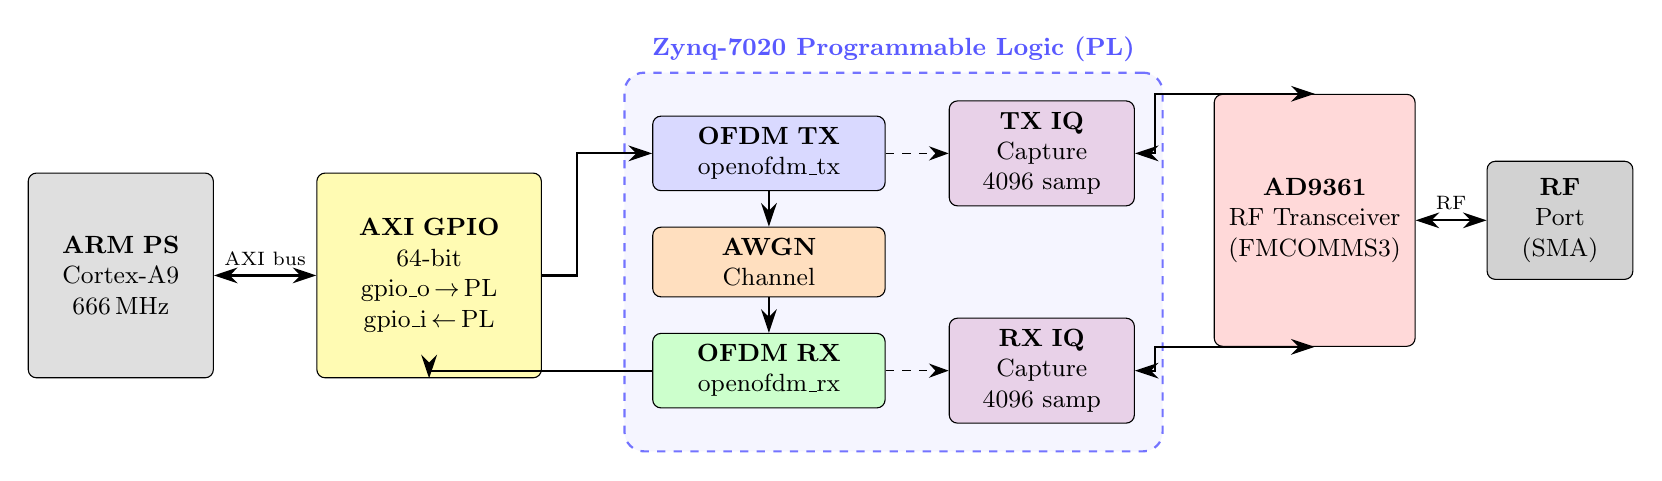
\begin{tikzpicture}[node distance=0.55cm and 1.1cm]
    %% --- ARM PS ---
    \node[blk={gray!25}{2.0cm}, minimum height=2.6cm, align=center] (ps)
      {\textbf{ARM PS}\\Cortex-A9\\666\,MHz};

    %% --- AXI GPIO ---
    \node[blk={yellow!30}{2.5cm}, minimum height=2.6cm, align=center,
          right=1.3cm of ps] (gpio)
      {\textbf{AXI GPIO}\\64-bit\\gpio\_o $\!\to\!$ PL\\gpio\_i $\!\leftarrow\!$ PL};

    %% --- PL blocks (stacked vertically) ---
    \node[blk={blue!15}{2.6cm}, align=center,
          right=1.4cm of gpio, yshift=1.55cm] (tx)
      {\textbf{OFDM TX}\\openofdm\_tx};
    \node[blk={orange!25}{2.6cm}, align=center, below=0.45cm of tx] (awgn)
      {\textbf{AWGN}\\Channel};
    \node[blk={green!20}{2.6cm}, align=center, below=0.45cm of awgn] (rx)
      {\textbf{OFDM RX}\\openofdm\_rx};

    %% --- IQ capture BRAMs ---
    \node[blk={violet!18}{2.0cm}, align=center,
          right=0.8cm of tx] (txcap)
      {\textbf{TX IQ}\\Capture\\4096 samp};
    \node[blk={violet!18}{2.0cm}, align=center,
          right=0.8cm of rx] (rxcap)
      {\textbf{RX IQ}\\Capture\\4096 samp};

    %% --- AD9361 ---
    \node[blk={red!15}{2.2cm}, minimum height=3.2cm, align=center,
          right=1.0cm of txcap, yshift=-0.85cm] (adi)
      {\textbf{AD9361}\\RF Transceiver\\(FMCOMMS3)};

    %% --- RF port ---
    \node[blk={gray!35}{1.5cm}, minimum height=1.5cm, align=center,
          right=0.9cm of adi] (rf)
      {\textbf{RF}\\Port\\(SMA)};

    %% === Connections ===
    %% PS <-> GPIO
    \draw[darr] (ps) -- node[above,font=\scriptsize]{AXI bus} (gpio);
    %% GPIO -> TX  and  RX -> GPIO (status)
    \draw[arr] (gpio.east) -- ++(0.45,0) |- (tx.west);
    \draw[arr] (rx.west)   -- ++(-0.45,0) -| (gpio.south);
    %% TX -> AWGN -> RX
    \draw[arr] (tx)   -- (awgn);
    \draw[arr] (awgn) -- (rx);
    %% IQ taps (dashed)
    \draw[sarr] (tx.east) -- (txcap.west);
    \draw[sarr] (rx.east) -- (rxcap.west);
    %% IQ caps <-> AD9361
    \draw[darr] (txcap.east) -- ++(0.25,0) |- (adi.north);
    \draw[darr] (rxcap.east) -- ++(0.25,0) |- (adi.south);
    %% AD9361 <-> RF
    \draw[darr, thick] (adi) -- node[above,font=\scriptsize]{RF} (rf);

    %% === PL bounding box ===
    \begin{scope}[on background layer]
      \node[draw=blue!55, dashed, thick, fill=blue!4, rounded corners=7pt,
            inner sep=10pt,
            fit=(tx)(awgn)(rx)(txcap)(rxcap),
            label={[blue!65,font=\small\bfseries]above:Zynq-7020 Programmable Logic (PL)}] {};
    \end{scope}
  \end{tikzpicture}%
  }
  \caption{High-level system architecture of the OFDM transceiver platform.}
  \label{fig:system_overview}
\end{figure}

The PS runs bare-metal C firmware that communicates with the PL over AXI GPIO buses. Transmitted OFDM packets are generated by the PL and optionally routed through an AWGN noise injection block before being passed to the AD9361 DAC and up-converted to an RF carrier. Received baseband IQ samples are captured from the AD9361 ADC and decoded by the OFDM receiver block in the PL. Results, status flags, and IQ sample data are returned to the PS via GPIO. A serial (UART) link connects the PS to a host PC running the Python GUI, which visualises performance metrics and controls system operation.

The report is organised as follows. Chapter~2 describes the hardware platform. Chapter~3 presents the HDL design. Chapter~4 details the NO-OS firmware. Chapter~5 describes the GUI application.

%% ============================================================
\chapter{HARDWARE}
%% ============================================================

\section{ZedBoard Architecture and Features}

The ZedBoard is an evaluation and development board for the Xilinx Zynq-7020 SoC, produced by Avnet and designed specifically to support rapid prototyping of embedded and FPGA-based applications. The Zynq-7020 integrates two ARM Cortex-A9 processors, operating at up to 866 MHz, tightly coupled with a 7-series FPGA fabric through a high-bandwidth AXI interconnect \cite{xilinx_zynq_trm}. This heterogeneous architecture eliminates the latency and bandwidth penalties of an external FPGA-to-processor interface bus, enabling the PS to directly control and observe signals in the PL domain.

Key hardware resources of the Zynq-7020 relevant to this project include:

\begin{table}[H]
  \centering
  \caption{Selected Zynq-7020 resources used in this project.}
  \label{tab:zynq_resources}
  \begin{tabular}{lll}
    \toprule
    \textbf{Resource} & \textbf{Available} & \textbf{Description} \\
    \midrule
    Cortex-A9 Cores      & 2        & Dual-core ARM processor, 866 MHz \\
    Look-Up Tables (LUT) & 53,200   & 6-input LUTs in the PL fabric \\
    Flip-Flops           & 106,400  & Registers for sequential logic \\
    Block RAM            & 140 $\times$ 36 Kbit & On-chip data storage \\
    DSP48E1 Slices       & 220      & Dedicated multiply-accumulate units \\
    PCIe / GTP Transceivers & 4    & High-speed serial interfaces \\
    AXI HP Ports         & 4        & High-performance DMA paths \\
    AXI GPIO Controllers & Multiple & PS-controlled I/O to PL \\
    \bottomrule
  \end{tabular}
\end{table}

The ZedBoard provides an FMC-LPC connector that exposes differential I/O pairs, single-ended GPIO, and power rails to an attached daughter card. This connector is used to interface the FMCOMMS3 radio module.

\begin{figure}[H]
  \centering
  \fbox{\parbox[c][6cm][c]{12cm}{\centering\small ZedBoard photograph: annotate FMC connector, JTAG, UART USB, SD slot, Ethernet, Zynq SoC location.}}
  \caption{ZedBoard development platform showing major interfaces.}
  \label{fig:zedboard_photo}
\end{figure}

\section{AD9361 RF Transceiver Architecture and Operation}

The AD9361 is a high-performance, highly integrated RF transceiver manufactured by Analog Devices Inc. It supports a frequency range of 70 MHz to 6 GHz with a signal bandwidth of up to 56 MHz and an internal 12-bit ADC/DAC resolution \cite{ad9361_ref_manual}. The device integrates transmit and receive chains, synthesisers, baseband filters, and power management in a single chip, making it the de-facto standard transceiver for software-defined radio (SDR) platforms.

The internal architecture of the AD9361 comprises the following signal processing stages:

\textbf{Receive Path:} RF signal enters via the LNA and is down-converted to in-phase (I) and quadrature (Q) baseband components by a quadrature demodulator. Variable gain amplifiers (VGAs) and adjustable baseband filters reduce out-of-band interference. The IQ signals are digitised by 12-bit pipeline ADCs and pass through digital decimation filters before appearing on the LVDS digital interface.

\textbf{Transmit Path:} Digital IQ data from the FPGA is provided over the LVDS interface, passed through interpolation filters, converted by 12-bit DACs, and up-converted to the desired RF carrier by an IQ modulator. A power amplifier driver stage delivers the output to the antenna port.

\textbf{Synthesisers:} Two fractional-N PLL synthesisers independently control the TX and RX local oscillator (LO) frequencies. This enables full-duplex or frequency-division duplex operation.

\begin{figure}[H]
  \centering
  \resizebox{\linewidth}{!}{%
  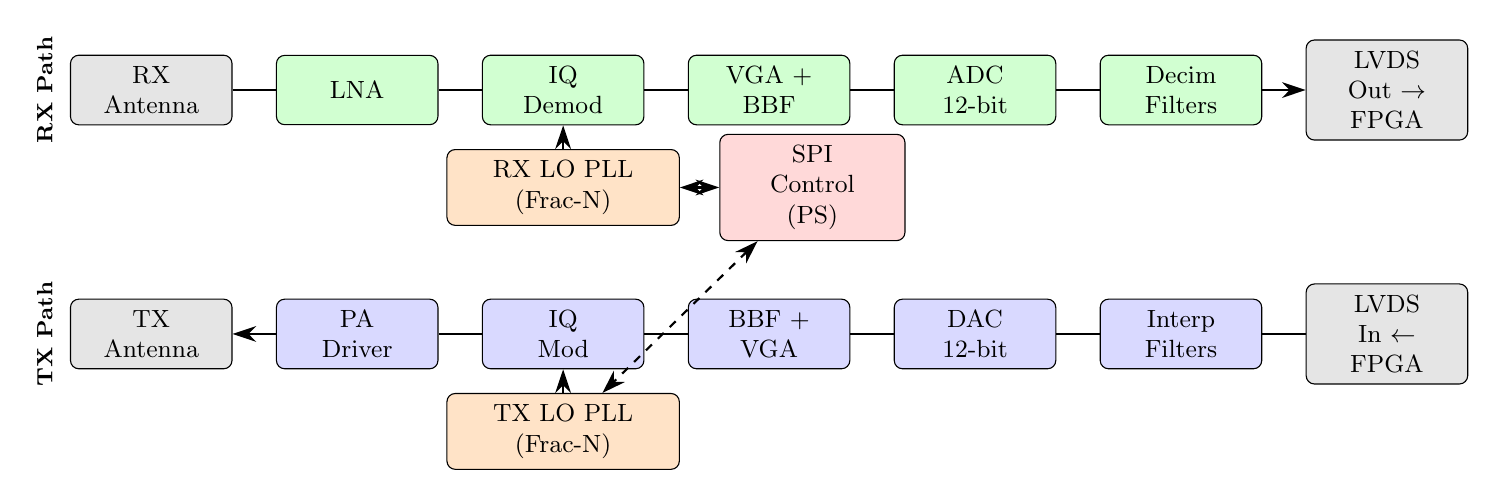
\begin{tikzpicture}[node distance=0.35cm and 0.55cm, font=\small]
    %% ---- RX chain (top row) ----
    \node[nblk={gray!20}]                          (rxant) {RX\\Antenna};
    \node[nblk={green!18},  right=of rxant]        (lna)   {LNA};
    \node[nblk={green!18},  right=of lna]          (mix)   {IQ\\Demod};
    \node[nblk={green!18},  right=of mix]          (vga)   {VGA +\\BBF};
    \node[nblk={green!18},  right=of vga]          (adc)   {ADC\\12-bit};
    \node[nblk={green!18},  right=of adc]          (dec)   {Decim\\Filters};
    \node[nblk={gray!20},   right=of dec]          (lvdsrx){LVDS\\Out $\to$ FPGA};

    %% ---- TX chain (bottom row, 2.2cm below) ----
    \node[nblk={gray!20},  below=2.2cm of rxant]   (txant) {TX\\Antenna};
    \node[nblk={blue!15},  right=of txant]         (pa)    {PA\\Driver};
    \node[nblk={blue!15},  right=of pa]            (iqmod) {IQ\\Mod};
    \node[nblk={blue!15},  right=of iqmod]         (bbftx) {BBF +\\VGA};
    \node[nblk={blue!15},  right=of bbftx]         (dac)   {DAC\\12-bit};
    \node[nblk={blue!15},  right=of dac]           (interp){Interp\\Filters};
    \node[nblk={gray!20},  right=of interp]        (lvdstx){LVDS\\In $\leftarrow$ FPGA};

    %% ---- LO PLL (centred between rows) ----
    \node[blk={orange!22}{2.6cm}, align=center,
          below=0.6cm of mix, yshift=0.3cm] (rxpll) {RX LO PLL\\(Frac-N)};
    \node[blk={orange!22}{2.6cm}, align=center,
          below=0.6cm of iqmod, yshift=0.3cm] (txpll) {TX LO PLL\\(Frac-N)};
    \node[blk={red!15}{2.0cm}, align=center,
          right=0.5cm of rxpll] (spi) {SPI\\Control\\(PS)};

    %% ---- RX arrows ----
    \draw[arr] (rxant)--(lna)--(mix)--(vga)--(adc)--(dec)--(lvdsrx);

    %% ---- TX arrows ----
    \draw[arr] (lvdstx)--(interp)--(dac)--(bbftx)--(iqmod)--(pa)--(txant);

    %% ---- LO feeds ----
    \draw[arr] (rxpll.north) -- (mix.south);
    \draw[arr] (txpll.north) -- (iqmod.south);

    %% ---- SPI ----
    \draw[darr, dashed] (spi) -- (rxpll);
    \draw[darr, dashed] (spi) -- (txpll);

    %% ---- Labels ----
    \node[font=\footnotesize\bfseries, left=0.1cm of rxant, rotate=90,
          anchor=south] {RX Path};
    \node[font=\footnotesize\bfseries, left=0.1cm of txant, rotate=90,
          anchor=south] {TX Path};
  \end{tikzpicture}%
  }
  \caption{Simplified internal architecture of the AD9361 RF transceiver.}
  \label{fig:ad9361_block}
\end{figure}

The AD9361 is controlled via a 4-wire SPI bus. Hundreds of internal registers configure carrier frequency, gain, bandwidth, sampling rate, interface timing, and calibration. In this project the AD9361 is configured for a 2.4 GHz carrier, 20 MSPS complex sampling rate, and 18 MHz analogue baseband filter bandwidth.

\section{Hardware Setup and System Architecture}

The FMCOMMS3 daughter card mounts directly onto the ZedBoard FMC-LPC connector and supplies the AD9361 with power from the board's 12 V rail. The FMC connector carries the LVDS data buses (P0 and P1), the SPI control lines, and auxiliary signals including GPIO and clock references. An SMA connector on the FMCOMMS3 provides the RF port; for loopback testing, a coaxial cable connects the TX SMA directly to the RX SMA.

\begin{figure}[H]
  \centering
  \fbox{\parbox[c][6cm][c]{12cm}{\centering\small Hardware setup photograph: ZedBoard + FMCOMMS3, RF cable loopback, USB-UART cable to host PC.}}
  \caption{Physical hardware setup: ZedBoard with FMCOMMS3 in RF loopback configuration.}
  \label{fig:hw_setup}
\end{figure}

\section{Communication Between ZedBoard and AD9361}

\subsection{SPI Configuration Interface}

All AD9361 register reads and writes are performed via SPI. The Zynq PS drives the SPI peripheral in master mode. On power-up, the NO-OS firmware executes a calibration sequence that configures the RF synthesisers, sets the ADC/DAC sample rates, adjusts the baseband filter bandwidth, and runs internal quadrature calibration algorithms to compensate for I/Q gain and phase mismatch. Detailed SPI transactions are managed by the ADI driver layer abstracted in the NO-OS software stack.

\subsection{LVDS Digital Data Interface}

Baseband IQ samples are transferred between the Zynq PL and the AD9361 over a dual-lane LVDS interface. Each lane carries 12-bit samples at DDR (double data rate), yielding an effective throughput of 2 $\times$ 12 bits $\times$ 2 (DDR) $\times$ f\textsubscript{sample} per direction. At 20 MSPS, this provides a comfortable margin for the 64-subcarrier OFDM signal. The ADI \texttt{axi\_ad9361} HDL core, instantiated in the PL block design, handles LVDS deserialisation and provides a parallel IQ bus to the signal processing logic.

\subsection{AXI GPIO Control Plane}

An AXI GPIO peripheral provides a 64-bit output register (\texttt{gpio\_o}) from the PS to the PL and a 64-bit input register (\texttt{gpio\_i}) from the PL to the PS. This control plane carries transmit/receive triggers, AWGN enable and gain settings, IQ capture index, and status/decode result flags. The bit field assignments are defined in the firmware header and the HDL top-level module and are described in detail in Chapters~3 and~4.

\section{Hardware Design Considerations}

Several practical hardware design decisions are worth noting:

\textbf{Clock domains:} The system operates with three principal clock domains—the AD9361 reference clock (40 MHz from an on-board oscillator), the baseband processing clock (\texttt{bb\_clk}, derived by the \texttt{axi\_clkgen} block), and the Zynq processing system clock (CPU at 666 MHz, AXI at 166 MHz). Signals crossing between domains require proper two-flip-flop synchronisers, which are implemented in the HDL.

\textbf{RF loopback path:} The coaxial loopback cable introduces a signal path attenuation and a small propagation delay. RF cable attenuation and connector losses are calibrated into the AGC loop of the AD9361 automatically.

\textbf{AWGN emulation:} The on-chip AWGN module enables repeatable noise experiments without requiring open-air propagation or controlled RF chambers. SNR is set digitally through the GPIO interface from the ARM firmware.

%% ============================================================
\chapter{HDL DESIGN}
%% ============================================================

\section{Overall HDL Architecture}

The HDL design is the heart of the physical-layer implementation. It is organised as a single top-level Verilog module, \texttt{system\_top.v}, that instantiates the Vivado block design (generated by \texttt{system\_bd.tcl}) alongside custom RTL modules. Figure~\ref{fig:hdl_arch} shows the top-level signal flow.

\begin{figure}[H]
  \centering
  \resizebox{0.9\linewidth}{!}{%
  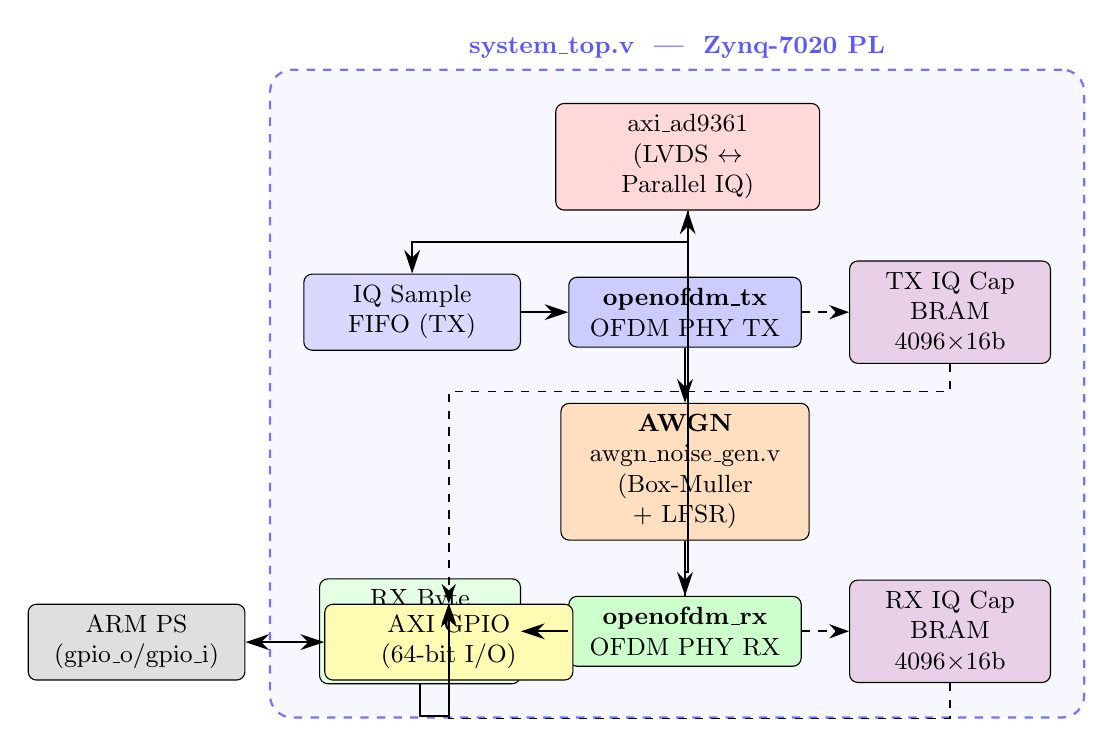
\begin{tikzpicture}[node distance=0.5cm and 0.7cm, font=\small]
    %% ---- Row 0: AD9361 interface ----
    \node[blk={red!15}{3.0cm}, align=center] (axiad) {axi\_ad9361\\(LVDS $\leftrightarrow$ Parallel IQ)};

    %% ---- Row 1: TX path ----
    \node[blk={blue!15}{2.4cm}, align=center, below=0.8cm of axiad, xshift=-3.5cm] (txfifo)
      {IQ Sample\\FIFO (TX)};
    \node[blk={blue!20}{2.6cm}, align=center, right=0.6cm of txfifo] (ofdmtx)
      {\textbf{openofdm\_tx}\\OFDM PHY TX};
    \node[blk={violet!18}{2.2cm}, align=center, right=0.6cm of ofdmtx] (txcap)
      {TX IQ Cap\\BRAM\\4096$\times$16b};

    %% ---- Row 2: AWGN ----
    \node[blk={orange!25}{2.8cm}, align=center, below=0.7cm of ofdmtx] (awgnblk)
      {\textbf{AWGN}\\awgn\_noise\_gen.v\\(Box-Muller + LFSR)};

    %% ---- Row 3: RX path ----
    \node[blk={green!20}{2.6cm}, align=center, below=0.7cm of awgnblk] (ofdmrx)
      {\textbf{openofdm\_rx}\\OFDM PHY RX};
    \node[blk={violet!18}{2.2cm}, align=center, right=0.6cm of ofdmrx] (rxcap)
      {RX IQ Cap\\BRAM\\4096$\times$16b};
    \node[blk={green!10}{2.2cm}, align=center, left=0.6cm of ofdmrx] (rxbuf)
      {RX Byte\\Buffer +\\Result Reg};

    %% ---- Row 4: GPIO + PS ----
    \node[blk={yellow!30}{2.8cm}, align=center, below=0.8cm of awgnblk, xshift=-3.0cm] (gpioip)
      {AXI GPIO\\(64-bit I/O)};
    \node[blk={gray!25}{2.4cm}, align=center, left=1.0cm of gpioip] (ps)
      {ARM PS\\(gpio\_o/gpio\_i)};

    %% === Signal flow ===
    %% AD9361 -> TX FIFO
    \draw[arr] (axiad.south) -- ++(0,-0.4) -| (txfifo.north);
    %% TX FIFO -> openofdm_tx
    \draw[arr] (txfifo) -- (ofdmtx);
    %% TX -> cap
    \draw[sarr] (ofdmtx.east) -- (txcap.west);
    %% TX -> AWGN
    \draw[arr] (ofdmtx.south) -- (awgnblk.north);
    %% AWGN -> RX
    \draw[arr] (awgnblk.south) -- (ofdmrx.north);
    %% RX -> cap
    \draw[sarr] (ofdmrx.east) -- (rxcap.west);
    %% RX -> result buf
    \draw[arr] (ofdmrx.west) -- (rxbuf.east);
    %% RX -> AD9361
    \draw[arr] (ofdmrx.north) -- ++(0,0.3) -| (axiad.south);
    %% result buf -> GPIO
    \draw[arr] (rxbuf.south) -- ++(0,-0.4) -| (gpioip.north);
    %% IQ caps -> GPIO
    \draw[sarr] (txcap.south) -- ++(0,-0.35) -| (gpioip.north);
    \draw[sarr] (rxcap.south) -- ++(0,-0.45) -| (gpioip.north);
    %% GPIO <-> PS
    \draw[darr] (gpioip) -- (ps);

    %% === PL box ===
    \begin{scope}[on background layer]
      \node[draw=blue!55, dashed, thick, fill=blue!3, rounded corners=8pt,
            inner sep=12pt,
            fit=(axiad)(txfifo)(ofdmtx)(txcap)(awgnblk)(ofdmrx)(rxcap)(rxbuf)(gpioip),
            label={[blue!65,font=\small\bfseries]above:system\_top.v \ --- \ Zynq-7020 PL}] {};
    \end{scope}
  \end{tikzpicture}%
  }
  \caption{Top-level HDL architecture showing major signal processing blocks.}
  \label{fig:hdl_arch}
\end{figure}

The block design, generated by the Vivado \texttt{system\_bd.tcl} script, contains the Zynq PS configuration, the \texttt{axi\_ad9361} data-plane interface, the \texttt{axi\_clkgen} clock generator, and the AXI GPIO peripheral. All custom DSP blocks are instantiated in \texttt{system\_top.v} outside the block design wrapper to maintain clarity and flexibility in simulation and synthesis.

The full project is built using a batch Tcl script (\texttt{build.tcl}) that creates the Vivado project, adds sources, synthesises, inserts an Integrated Logic Analyser (ILA) debug core for observability, and runs implementation and bitstream generation in a single command.

\begin{figure}[H]
  \centering
  \fbox{\parbox[c][6cm][c]{12cm}{\centering\small Vivado block design canvas screenshot: Zynq PS, axi\_ad9361, axi\_clkgen, AXI GPIO, interconnects.}}
  \caption{Vivado block design (system\_bd) showing IP core connections.}
  \label{fig:vivado_bd}
\end{figure}

\section{OFDM Transmitter}

\subsection{Purpose and Operation}

The OFDM transmitter is implemented using the open-source \texttt{openofdm\_tx} IP core \cite{openofdm}. The transmitter accepts a stream of payload bytes and produces a baseband IQ sample stream conforming to the IEEE 802.11a PHY framing structure. The transmission process proceeds through the following pipeline stages:

\begin{enumerate}[noitemsep]
  \item \textbf{PLCP header construction:} The scrambled PLCP preamble (short training field, long training field, SIGNAL field) is prepended to the payload.
  \item \textbf{Scrambling:} Data bits are XOR-scrambled with a 127-bit PN sequence to prevent long runs of identical bits.
  \item \textbf{Convolutional encoding:} A rate-1/2 convolutional code with constraint length $K=7$ and generator polynomials $g_0 = 1011011_2$, $g_1 = 1111001_2$ provides forward error correction. Puncturing raises the effective code rate to 2/3 or 3/4 for higher MCS values.
  \item \textbf{Interleaving:} Coded bits are block-interleaved across sub-carriers and over multiple OFDM symbols to distribute burst errors.
  \item \textbf{Sub-carrier mapping:} Interleaved bits are mapped to BPSK, QPSK, 16-QAM, or 64-QAM constellation points and loaded onto the 48 data sub-carriers. Four pilot sub-carriers at indices $\pm 7$ and $\pm 21$ carry known BPSK symbols.
  \item \textbf{64-point IFFT:} An IFFT converts the frequency-domain sub-carrier vector to a time-domain OFDM symbol.
  \item \textbf{Cyclic prefix insertion:} The last 16 samples of each IFFT output are prepended as the guard interval (cyclic prefix) to eliminate inter-symbol interference from channel delay spread up to $\sim$800 ns.
\end{enumerate}

\begin{figure}[H]
  \centering
  \resizebox{\linewidth}{!}{%
  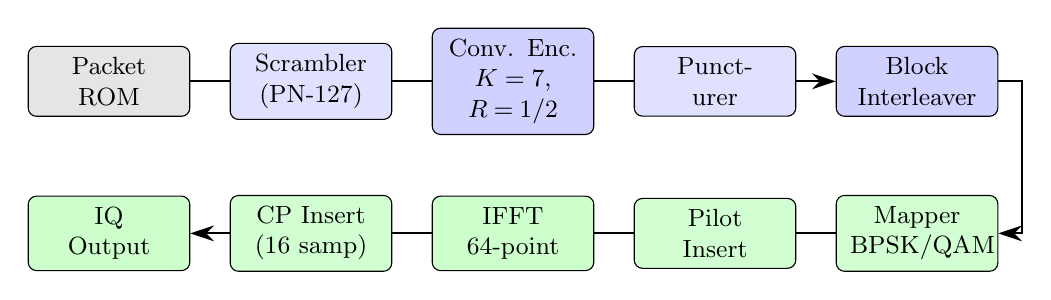
\begin{tikzpicture}[node distance=0.4cm and 0.5cm, font=\small]
    %% ---- Row 1 ----
    \node[nblk={gray!20}]                       (rom)  {Packet\\ROM};
    \node[nblk={blue!12}, right=of rom]         (scr)  {Scrambler\\(PN-127)};
    \node[nblk={blue!18}, right=of scr]         (enc)  {Conv. Enc.\\$K\!=\!7$, $R\!=\!1/2$};
    \node[nblk={blue!12}, right=of enc]         (pun)  {Punct-\\urer};
    \node[nblk={blue!18}, right=of pun]         (intl) {Block\\Interleaver};

    %% ---- Row 2 ----
    \node[nblk={green!20}, below=1.0cm of rom]  (iqout){IQ\\Output};
    \node[nblk={green!18}, right=of iqout]      (cpins){CP Insert\\(16 samp)};
    \node[nblk={green!20}, right=of cpins]      (ifft) {IFFT\\64-point};
    \node[nblk={green!18}, right=of ifft]       (pilot){Pilot\\Insert};
    \node[nblk={green!18}, right=of pilot]      (map)  {Mapper\\BPSK/QAM};

    %% Row 1 flow
    \draw[arr] (rom)--(scr)--(enc)--(pun)--(intl);
    %% Row 1 end -> Row 2 start (bent arrow)
    \draw[arr] (intl.east) -- ++(0.3,0) |- (map.east);
    %% Row 2 flow (right to left)
    \draw[arr] (map)--(pilot)--(ifft)--(cpins)--(iqout);
  \end{tikzpicture}%
  }
  \caption{OFDM transmitter processing pipeline.}
  \label{fig:tx_pipeline}
\end{figure}

\subsection{Interaction with System}

The PS asserts a one-cycle \texttt{phy\_tx\_start} pulse via GPIO to initiate a transmission. The data payload is stored in a packet ROM (\texttt{tx\_packet\_rom\_mcs.v}), addressed by a counter driven by the transmitter's data-ready handshake. The transmitter signals completion via the \texttt{phy\_tx\_done} flag read back by the PS through \texttt{gpio\_i}. The resulting 16-bit signed IQ sample pairs are routed to the AWGN channel module and simultaneously captured in the TX IQ buffer.

\section{OFDM Receiver}

\subsection{Purpose and Operation}

The OFDM receiver is implemented by the \texttt{openofdm\_rx} IP core \cite{openofdm}. It operates on the IQ sample stream emerging from the AWGN channel module and performs the following steps:

\begin{enumerate}[noitemsep]
  \item \textbf{Packet detection:} A sliding-window energy detector identifies the short training sequence preamble.
  \item \textbf{Coarse frequency offset correction:} The periodicity of the short preamble is exploited to estimate and compensate for carrier frequency offset (CFO).
  \item \textbf{FFT window alignment:} The long training sequence (LTF) provides fine timing synchronisation and the FFT window start position.
  \item \textbf{Channel estimation:} The known LTF sub-carrier symbols are used to estimate the complex channel coefficient for each sub-carrier.
  \item \textbf{64-point FFT:} Each OFDM symbol, after cyclic prefix removal, is transformed to the frequency domain.
  \item \textbf{Single-tap equalisation:} Each sub-carrier is divided by its estimated channel coefficient.
  \item \textbf{Sub-carrier demapping:} Equalised symbols are de-mapped according to the modulation order decoded from the SIGNAL field.
  \item \textbf{De-interleaving, Viterbi decoding, de-scrambling:} The received coded bits are processed in reverse to recover the original payload bytes.
  \item \textbf{FCS checking:} The 32-bit IEEE CRC is verified and the result is reported via the \texttt{rx\_fcs\_ok} flag.
\end{enumerate}

\begin{figure}[H]
  \centering
  \resizebox{\linewidth}{!}{%
  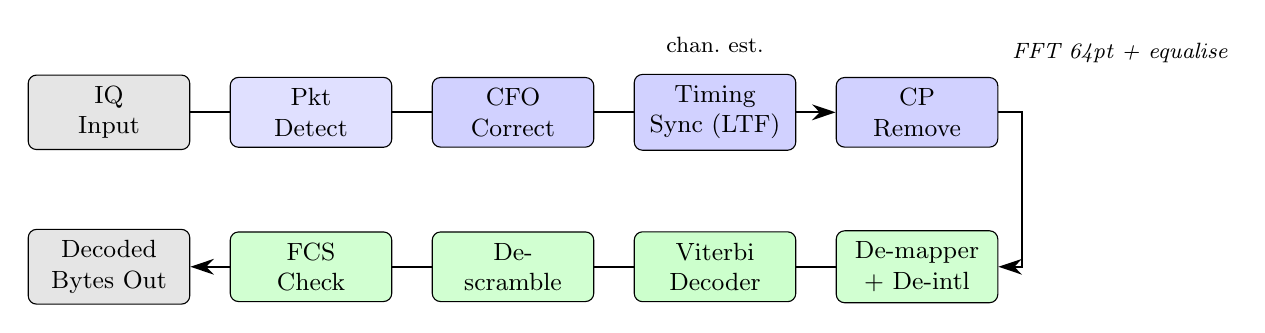
\begin{tikzpicture}[node distance=0.4cm and 0.5cm, font=\small]
    %% ---- Row 1 ----
    \node[nblk={gray!20}]                        (iqin) {IQ\\Input};
    \node[nblk={blue!12}, right=of iqin]         (pdet) {Pkt\\Detect};
    \node[nblk={blue!18}, right=of pdet]         (cfo)  {CFO\\Correct};
    \node[nblk={blue!18}, right=of cfo]          (tsyn) {Timing\\Sync (LTF)};
    \node[nblk={blue!18}, right=of tsyn]         (cprem){CP\\Remove};

    %% ---- Row 2 ----
    \node[nblk={gray!20}, below=1.0cm of iqin]   (bout) {Decoded\\Bytes Out};
    \node[nblk={green!18}, right=of bout]        (fcs)  {FCS\\Check};
    \node[nblk={green!18}, right=of fcs]         (dscr) {De-\\scramble};
    \node[nblk={green!20}, right=of dscr]        (vit)  {Viterbi\\Decoder};
    \node[nblk={green!18}, right=of vit]         (dmap) {De-mapper\\+ De-intl};

    %% Row 1 flow
    \draw[arr] (iqin)--(pdet)--(cfo)--(tsyn)--(cprem);
    %% Row 1 end -> FFT -> equalise -> Row 2
    \draw[arr] (cprem.east) -- ++(0.3,0) |- (dmap.east);
    %% Row 2 flow (right to left)
    \draw[arr] (dmap)--(vit)--(dscr)--(fcs)--(bout);

    %% Channel estimate annotation
    \node[font=\footnotesize, above=0.15cm of tsyn] {chan.\ est.};
    \node[font=\footnotesize\itshape, above right=0.05cm and 0.05cm of cprem]
      {FFT 64pt + equalise};
  \end{tikzpicture}%
  }
  \caption{OFDM receiver processing pipeline.}
  \label{fig:rx_pipeline}
\end{figure}

\subsection{Interaction with System}

Decoded bytes are presented on an 8-bit output bus with a one-cycle \texttt{rx\_byte\_out\_strobe} valid signal. These are serialised into a result register accessible via \texttt{gpio\_i}. The \texttt{rx\_fcs\_out\_strobe} and \texttt{rx\_fcs\_ok} flags notify the PS of the end and validity of each received packet. The PS reads the decoded bytes and computes the Hamming distance against the known transmitted payload to derive the BER.

\section{AWGN Channel Module}

\subsection{Purpose and Operation}

The AWGN channel module (\texttt{awgn\_noise\_gen.v}) sits between the transmitter output and the receiver input, providing a controlled noise injection mechanism for in-the-loop BER characterisation without an RF link. The module generates complex Gaussian noise samples using a Box-Muller transform applied to pairs of uniform pseudorandom numbers produced by a linear feedback shift register (LFSR).

The variance of the noise (and hence the effective SNR) is controlled by a scaling factor that is set via the GPIO control bus from the PS firmware. When the AWGN module is disabled, the transmitter IQ samples pass through unmodified. The IQ sample FIFO (\texttt{iq\_sample\_fifo.v}) at the channel input buffers the transmitter output to handle the clock-cycle latency introduced by the noise computation pipeline.

\begin{figure}[H]
  \centering
  \resizebox{0.92\linewidth}{!}{%
  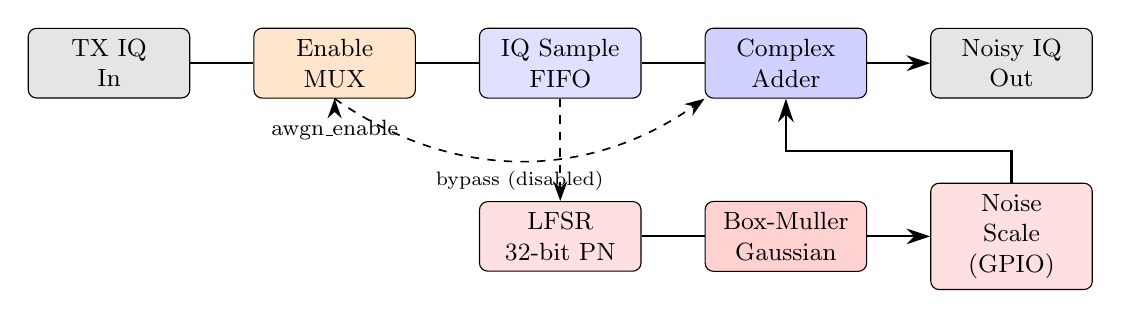
\begin{tikzpicture}[node distance=0.5cm and 0.8cm, font=\small]
    %% ---- Main signal path (top row) ----
    \node[nblk={gray!20}]                          (txiq) {TX IQ\\In};
    \node[nblk={orange!20}, right=of txiq]         (mux)  {Enable\\MUX};
    \node[nblk={blue!12},   right=of mux]          (fifo) {IQ Sample\\FIFO};
    \node[nblk={blue!18},   right=of fifo]         (add)  {Complex\\Adder};
    \node[nblk={gray!20},   right=of add]          (out)  {Noisy IQ\\Out};

    %% ---- Noise generation path (bottom row) ----
    \node[nblk={red!12},    below=1.3cm of fifo]   (lfsr) {LFSR\\32-bit PN};
    \node[nblk={red!18},    right=of lfsr]         (bm)   {Box-Muller\\Gaussian};
    \node[nblk={red!12},    right=of bm]           (scl)  {Noise\\Scale\\(GPIO)};

    %% ---- AWGN enable (control) ----
    \node[font=\footnotesize, below=0.15cm of mux] (enctrl) {awgn\_enable};

    %% ---- Main path arrows ----
    \draw[arr] (txiq)--(mux)--(fifo)--(add)--(out);

    %% ---- Noise path arrows ----
    \draw[arr] (lfsr)--(bm)--(scl);
    \draw[arr] (scl.north) -- ++(0,0.4) -| (add.south);

    %% ---- Enable dashed ----
    \draw[sarr] (enctrl) -- (mux.south);

    %% ---- LFSR starts from TX path (clock) ----
    \draw[sarr] (fifo.south) -- ++(0,-0.4) -| (lfsr.north);

    %% bypass arrow when AWGN disabled
    \draw[sarr, bend right=35] (mux.south) to
      node[below, font=\scriptsize]{bypass (disabled)} (add.south west);
  \end{tikzpicture}%
  }
  \caption{AWGN channel emulation module architecture.}
  \label{fig:awgn_module}
\end{figure}

\subsection{SNR Setting Procedure}

The relationship between the GPIO noise-scale register value and the effective baseband SNR is characterised during calibration. The firmware encodes the desired SNR in dB into a linear noise amplitude scale, compensating for the known transmit signal power. A look-up table in the firmware maps discrete SNR steps to register values.

\section{IQ Capture Buffers}

To provide the GUI with IQ sample data for visualisation, two independent capture buffers are implemented in block RAM within the PL.

\subsection{TX IQ Capture Buffer}

A 4096-deep $\times$ 16-bit block RAM array captures I and Q samples from the OFDM transmitter output on the \texttt{bb\_clk} domain. Samples are written sequentially during the transmit burst, up to a configurable capture limit. An 12-bit index register, synchronised from the \texttt{bb\_clk} domain to the PS's AXI GPIO read cycle, selects which sample to present on the read-data outputs \texttt{gpio\_i[31:16]} (I) and \texttt{gpio\_i[47:32]} (Q).

\subsection{RX IQ Capture Buffer}

An equivalent buffer captures samples on the \texttt{l\_clk} domain (the AD9361 receive clock). Block RAM inference is used with registered (synchronous) read ports to satisfy Vivado timing requirements. The GPIO-driven address bus is synchronised into the \texttt{l\_clk} domain through a two-flip-flop synchroniser before addressing the read port.

\begin{figure}[H]
  \centering
  \resizebox{\linewidth}{!}{%
  \begin{tikzpicture}[node distance=0.45cm and 0.7cm, font=\small]
    %% ====================== TX path (top) ======================
    \node[nblk={blue!15}]                           (txiq)   {TX IQ\\(bb\_clk)};
    \node[nblk={blue!20}, right=of txiq]            (txwr)   {BRAM Write\\Port (4096)};
    \node[nblk={blue!15}, right=of txwr]            (txbram) {TX IQ BRAM\\4096$\times$32b};
    \node[nblk={blue!20}, right=of txbram]          (txrd)   {BRAM Read\\Port (sync)};
    \node[nblk={gray!20}, right=of txrd]            (txout)  {gpio\_i\\[I, Q]};

    %% TX address sync path
    \node[nblk={orange!20}, below=0.7cm of txbram]  (txsyn)  {2-FF Sync\\(bb\_clk)};
    \node[nblk={yellow!30}, left=0.7cm of txsyn]    (gpioout){gpio\_o\\iq\_idx[11:0]};

    %% ====================== RX path (bottom) ======================
    \node[nblk={green!15}, below=2.2cm of txiq]     (rxiq)   {RX IQ\\(l\_clk)};
    \node[nblk={green!20}, right=of rxiq]           (rxwr)   {BRAM Write\\Port (4096)};
    \node[nblk={green!15}, right=of rxwr]           (rxbram) {RX IQ BRAM\\4096$\times$32b};
    \node[nblk={green!20}, right=of rxbram]         (rxrd)   {BRAM Read\\Port (sync)};
    \node[nblk={gray!20},  right=of rxrd]           (rxout)  {gpio\_i\\[I, Q]};

    %% RX address sync path
    \node[nblk={orange!20}, below=0.7cm of rxbram]  (rxsyn)  {2-FF Sync\\(l\_clk)};

    %% === TX arrows ===
    \draw[arr] (txiq)--(txwr)--(txbram)--(txrd)--(txout);
    \draw[arr] (gpioout)--(txsyn);
    \draw[arr] (txsyn.north) -- (txbram.south);

    %% === RX arrows ===
    \draw[arr] (rxiq)--(rxwr)--(rxbram)--(rxrd)--(rxout);
    \draw[arr] (gpioout.south) -- ++(0,-0.3) |- (rxsyn.west);
    \draw[arr] (rxsyn.north) -- (rxbram.south);

    %% Clock domain labels
    \node[font=\footnotesize\itshape, above=0.05cm of txiq, xshift=1cm]
      {\textit{bb\_clk domain}};
    \node[font=\footnotesize\itshape, above=0.05cm of rxiq, xshift=1cm]
      {\textit{l\_clk domain}};
  \end{tikzpicture}%
  }
  \caption{IQ capture buffer architecture showing dual-clock synchronisation.}
  \label{fig:iq_capture}
\end{figure}

\section{Data Flow and Signal Processing Chain}

Figure~\ref{fig:dataflow} illustrates the complete data flow from packet generation to BER reporting:

\begin{figure}[H]
  \centering
  \resizebox{\linewidth}{!}{%
  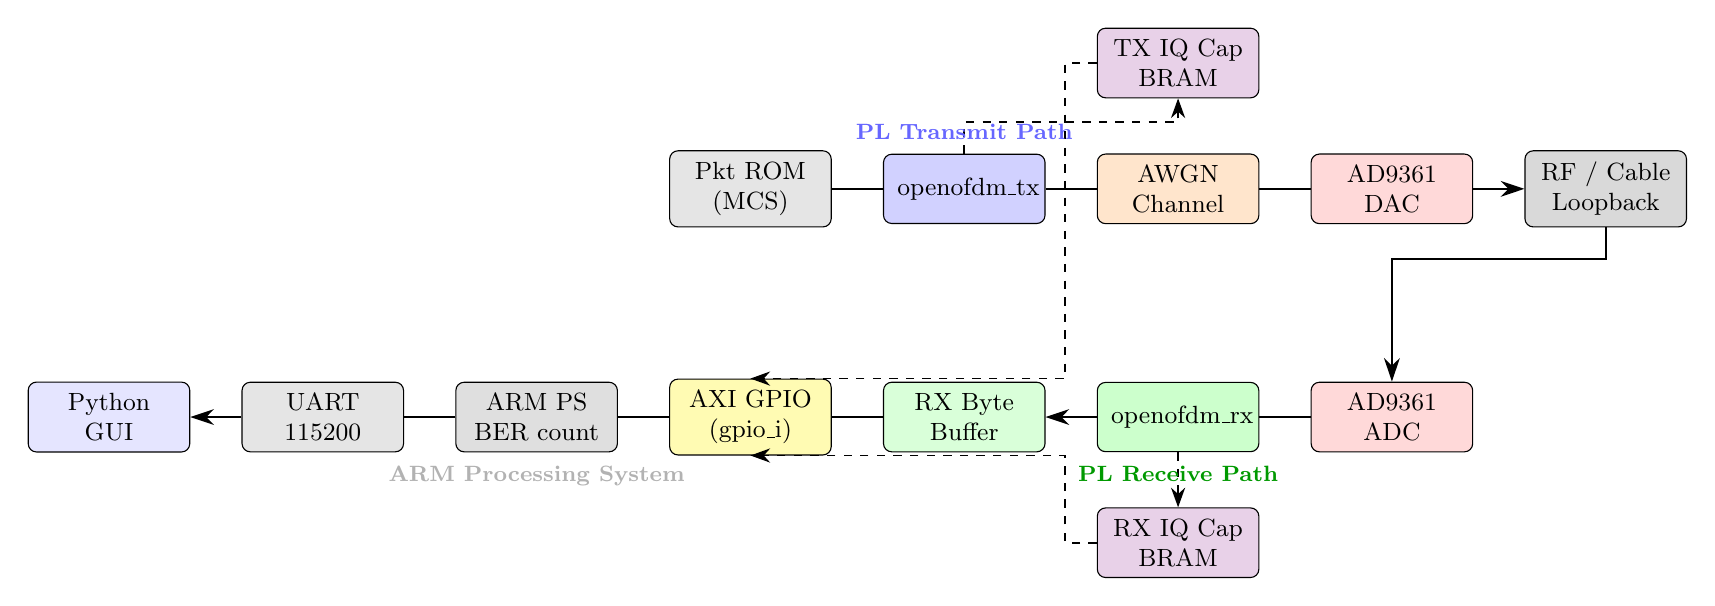
\begin{tikzpicture}[node distance=0.45cm and 0.65cm, font=\small]
    %% ====================== Layer 1: TX (PL) ======================
    \node[nblk={gray!20}]                            (rom)   {Pkt ROM\\(MCS)};
    \node[nblk={blue!18},  right=of rom]             (otx)   {openofdm\_tx};
    \node[nblk={orange!20},right=of otx]             (awgn)  {AWGN\\Channel};
    \node[nblk={red!15},   right=of awgn]            (dac)   {AD9361\\DAC};
    \node[nblk={gray!30},  right=of dac]             (rfcoax){RF / Cable\\Loopback};

    %% TX IQ capture branch
    \node[nblk={violet!18}, above=0.7cm of awgn]     (txcap) {TX IQ Cap\\BRAM};

    %% ====================== Layer 2: RX (PL) ======================
    \node[nblk={red!15},   below=2.0cm of dac]       (adc)   {AD9361\\ADC};
    \node[nblk={green!20}, left=of adc]              (orx)   {openofdm\_rx};
    \node[nblk={green!15}, left=of orx]              (rxbuf) {RX Byte\\Buffer};
    \node[nblk={violet!18},below=0.7cm of orx]       (rxcap) {RX IQ Cap\\BRAM};

    %% ====================== Layer 3: PS + GUI ======================
    \node[nblk={yellow!30}, left=of rxbuf]           (gpioblk){AXI GPIO\\(gpio\_i)};
    \node[nblk={gray!25},   left=of gpioblk]         (ps)    {ARM PS\\BER count};
    \node[nblk={gray!20},   left=of ps]              (uart)  {UART\\115200};
    \node[nblk={blue!10},   left=of uart]            (gui)   {Python\\GUI};

    %% === TX flow ===
    \draw[arr] (rom)--(otx)--(awgn)--(dac)--(rfcoax);
    \draw[sarr] (otx.north) -- ++(0,0.4) -| (txcap.south);
    %% RF -> ADC
    \draw[arr] (rfcoax.south) -- ++(0,-0.4) -| (adc.north);
    %% ADC -> RX
    \draw[arr] (adc)--(orx)--(rxbuf);
    \draw[sarr] (orx.south) -- ++(0,-0.4) -| (rxcap.north);
    %% RX -> PS -> GUI
    \draw[arr] (rxbuf)--(gpioblk)--(ps)--(uart)--(gui);
    %% IQ caps -> GPIO
    \draw[sarr] (txcap.west) -- ++(-0.4,0) |- (gpioblk.north);
    \draw[sarr] (rxcap.west) -- ++(-0.4,0) |- (gpioblk.south);

    %% Labels
    \node[font=\footnotesize\bfseries\color{blue!60}, above=0.05cm of otx]
      {PL Transmit Path};
    \node[font=\footnotesize\bfseries\color{green!60!black}, below=0.05cm of orx]
      {PL Receive Path};
    \node[font=\footnotesize\bfseries\color{gray!60}, below=0.05cm of ps]
      {ARM Processing System};
  \end{tikzpicture}%
  }
  \caption{End-to-end data flow diagram.}
  \label{fig:dataflow}
\end{figure}

\section{Interfaces and Communication Blocks}

\subsection{AXI GPIO Bit-Field Assignments}

The 64-bit \texttt{gpio\_o} (PS $\to$ PL) and \texttt{gpio\_i} (PL $\to$ PS) registers carry all control and status information. Key assignments are summarised in Table~\ref{tab:gpio_map}.

\begin{table}[H]
  \centering
  \caption{Selected AXI GPIO bit-field assignments.}
  \label{tab:gpio_map}
  \begin{tabular}{lllp{5.5cm}}
    \toprule
    \textbf{Register} & \textbf{Bit(s)} & \textbf{Name} & \textbf{Description} \\
    \midrule
    gpio\_o & 0     & phy\_tx\_start    & One-cycle TX trigger \\
    gpio\_o & 1     & awgn\_enable      & Enable AWGN module \\
    gpio\_o & 6:2   & awgn\_gain        & Noise scale (5-bit) \\
    gpio\_o & 7     & iq\_sel           & 0 = TX buffer, 1 = RX buffer \\
    gpio\_o & 18:7  & iq\_idx           & 12-bit sample index \\
    \midrule
    gpio\_i & 0     & phy\_tx\_done     & TX complete flag \\
    gpio\_i & 1     & rx\_fcs\_ok       & FCS pass/fail \\
    gpio\_i & 2     & rx\_pkt\_hdr\_ok  & Header decode valid \\
    gpio\_i & 3     & rx\_fcs\_strobe   & End-of-packet indicator \\
    gpio\_i & 15:8  & rx\_byte\_out     & Decoded byte \\
    gpio\_i & 16    & rx\_byte\_strobe  & Byte valid \\
    gpio\_i & 31:17 & iq\_data\_i       & IQ I sample (15-bit) \\
    gpio\_i & 47:32 & iq\_data\_q       & IQ Q sample (16-bit) \\
    \bottomrule
  \end{tabular}
\end{table}

\subsection{Packet ROM}

The \texttt{tx\_packet\_rom\_mcs.v} and \texttt{tx\_packet\_rom\_ht\_mcs.v} modules implement synchronous ROMs containing pre-computed PSDU payloads for each supported MCS. The transmitted bytes consist of a known pseudo-random sequence so that the receiver can compute exact BER by comparison.

\section{Integration Process}

The Vivado project is created and built entirely from the \texttt{build.tcl} batch script. The script:

\begin{enumerate}[noitemsep]
  \item Deletes any prior project directory to ensure a clean state.
  \item Creates a Vivado project targeting the \texttt{xc7z020clg484-1} device.
  \item Points the IP catalogue to the pre-built ADI HDL library.
  \item Sources \texttt{system\_bd.tcl} to generate the block design.
  \item Adds all RTL sources and XCI files.
  \item Sets include paths for shared header files.
  \item Launches synthesis with 12 parallel jobs.
  \item Opens the synthesised design and inserts an ILA core with ten probes for runtime signal capture.
  \item Launches implementation and bitstream generation.
  \item Exports the hardware platform as a \texttt{.xsa} file for use by Vitis.
\end{enumerate}

\begin{figure}[H]
  \centering
  \fbox{\parbox[c][5cm][c]{12cm}{\centering\small Vivado implementation report screenshot: device utilisation summary table (LUT, FF, BRAM, DSP percentages).}}
  \caption{Vivado implementation utilisation report for the synthesised design.}
  \label{fig:utilisation}
\end{figure}

\section{System Timing and Synchronization}

Correct operation of the multi-clock system requires that all inter-domain signal crossings are synchronised. The design uses the following strategies:

\textbf{Control signals (PS $\to$ PL):} Slow-changing GPIO bits cross from the AXI clock to \texttt{bb\_clk} and \texttt{l\_clk} through standard two-flip-flop synchronisers. The IQ index and AWGN gain are treated as static values during a burst, so multi-bit bus synchronisation by settling is acceptable.

\textbf{Status pulses (PL $\to$ PS):} Level signals (\texttt{phy\_tx\_done}, \texttt{rx\_fcs\_ok}) are latched in the destination domain and cleared by the PS. Strobe pulses that must cross domains are stretched to at least three destination-clock cycles before re-sampling.

\textbf{ILA debug core:} The ILA is clocked from \texttt{bb\_clk}, probing the transmitter output IQ and key receiver status signals. This allows real-time waveform capture through the Vivado Hardware Manager over JTAG without interrupting the running firmware.

%% ============================================================
\chapter{NO-OS SOFTWARE}
%% ============================================================

\section{Introduction to the Analog Devices NO-OS Framework}

The Analog Devices NO-OS framework is an open-source bare-metal software platform designed to initialise and operate ADI mixed-signal ICs on embedded systems without requiring a real-time operating system \cite{adi_noos}. The framework provides hardware abstraction layers (HALs) for SPI, I\textsuperscript{2}C, GPIO, and timer peripherals, and includes complete device drivers for the AD9361. By targeting the Zynq PS via Xilinx Standalone BSP libraries, the firmware achieves deterministic timing without the overhead of task scheduling.

The firmware for this project is structured as a single C translation unit (\texttt{main.c}) of approximately 2000 lines, compiled with \texttt{arm-none-eabi-gcc} and linked against the Xilinx Standalone BSP. The binary is loaded from an SD card or flashed via JTAG using Vitis.

\section{System Initialization}

On power-up or reset, the firmware performs the following initialisation sequence:

\begin{enumerate}[noitemsep]
  \item \textbf{Cache and MMU configuration:} The Cortex-A9 caches and memory management unit are configured by the BSP startup code.
  \item \textbf{AD9361 SPI initialisation:} The ADI driver initialises the SPI peripheral and verifies communication with the AD9361 by reading its product identification register.
  \item \textbf{RF parameter loading:} A pre-defined \texttt{AD9361\_InitParam} structure is passed to \texttt{ad9361\_init()}, specifying carrier frequency (2.4 GHz), sampling rate (20 MSPS), LO frequency, filter bandwidth, and interface parameters.
  \item \textbf{Calibration sequences:} The AD9361 driver automatically executes internal calibration routines including baseband DC offset calibration, RF DC offset calibration, quadrature calibration, and RSSI calibration.
  \item \textbf{GPIO initialisation:} The AXI GPIO peripheral addresses are mapped and initial control values are written.
  \item \textbf{UART initialisation:} The PS UART is configured at 115200 baud, 8N1 for serial communication with the host PC.
  \item \textbf{CLI launch:} Control is passed to the command-line interface (CLI) main loop.
\end{enumerate}

\begin{figure}[H]
  \centering
  \fbox{\parbox[c][5cm][c]{12cm}{\centering\small Terminal output screenshot: AD9361 initialisation log showing register writes, calibration pass messages, and CLI prompt.}}
  \caption{AD9361 initialisation and calibration log as seen from the serial console.}
  \label{fig:init_log}
\end{figure}

\section{RF Configuration Procedures}

All RF parameters are configured through wrapper functions around the ADI AD9361 driver API. The key configuration calls are summarised below:

\begin{lstlisting}[language=C, caption={RF configuration call sequence (excerpt from main.c).}]
/* Set RX LO frequency */
ad9361_set_rx_lo_freq(ad9361_phy, rx_lo_hz);

/* Set TX LO frequency */
ad9361_set_tx_lo_freq(ad9361_phy, tx_lo_hz);

/* Set sampling rate (same for TX and RX) */
ad9361_set_rx_sampling_freq(ad9361_phy, sample_rate_hz);
ad9361_set_tx_sampling_freq(ad9361_phy, sample_rate_hz);

/* Set analogue bandwidth */
ad9361_set_rx_rf_bandwidth(ad9361_phy, bw_hz);
ad9361_set_tx_rf_bandwidth(ad9361_phy, bw_hz);

/* Set TX attenuation (0 = maximum power) */
ad9361_set_tx_attenuation(ad9361_phy, 0, tx_atten_mdb);
\end{lstlisting}

All configurable parameters (LO frequency, sampling rate, attenuation) are adjustable at runtime through CLI commands without requiring firmware recompilation.

\section{CLI Structure}

The CLI is a blocking loop that reads newline-terminated command strings from the UART, tokenises them on white space, and dispatches to the appropriate handler function. The general structure is shown in Figure~\ref{fig:cli_flowchart}.

\begin{figure}[H]
  \centering
  \resizebox{0.72\linewidth}{!}{%
  \begin{tikzpicture}[node distance=0.55cm and 1.0cm, font=\small]
    \node[term]                                      (start)  {Firmware Start};
    \node[blk={blue!10}{3.4cm}, below=of start]      (read)   {Read UART line\\(blocking)};
    \node[blk={blue!10}{3.4cm}, below=of read]       (tok)    {Tokenise:\\cmd + args};
    \node[dec, below=of tok]                         (match)  {Known\\cmd?};
    \node[blk={green!18}{3.6cm}, right=2.0cm of match](exec)  {Execute handler\\(TX/RX/LOOP/SNR/\\MCS/SWEEP/CAPIQ/\\PARAM/HELP)};
    \node[blk={red!10}{3.4cm},   left=2.0cm of match] (unk)  {Print\\``Unknown cmd''};
    \node[blk={orange!15}{3.4cm}, below=1.1cm of match](emit) {Emit \texttt{\#\#TAG}\\structured response};

    %% Arrows
    \draw[arr] (start)--(read)--(tok)--(match);
    \draw[arr] (match.east) -- node[above,font=\scriptsize]{Yes} (exec.west);
    \draw[arr] (match.west) -- node[above,font=\scriptsize]{No}  (unk.east);
    \draw[arr] (exec.south) -- ++(0,-0.4) -| (emit.east);
    \draw[arr] (unk.south)  -- ++(0,-0.6) -| (emit.west);
    %% Loop back
    \draw[arr] (emit.south) -- ++(0,-0.4) -- ++(3.2,0)
               |- node[right,font=\scriptsize]{loop} (read.east);
  \end{tikzpicture}%
  }
  \caption{CLI command dispatch flowchart.}
  \label{fig:cli_flowchart}
\end{figure}

The firmware embeds a structured line protocol: every machine-readable output line is prefixed with \texttt{\#\#} so that the GUI parser can distinguish firmware telemetry from human-readable console messages. Key message types are listed in Table~\ref{tab:serial_protocol}.

\begin{table}[H]
  \centering
  \caption{Structured serial protocol messages emitted by the firmware.}
  \label{tab:serial_protocol}
  \begin{tabular}{lp{9cm}}
    \toprule
    \textbf{Prefix} & \textbf{Payload and meaning} \\
    \midrule
    \texttt{\#\#PKT}        & Packet event: \texttt{pkt=N fcs=0/1 hdr=0/1 ber=F snr=S mcs=M} \\
    \texttt{\#\#PKT\_DATA}  & Raw bytes: \texttt{pkt=N fcs=0/1 hdr=0/1 hex=B0 B1 ... Bn} \\
    \texttt{\#\#IQ\_BURST}  & IQ sample burst: \texttt{is\_tx=0/1 n=N data=I0,Q0,I1,Q1,...} \\
    \texttt{\#\#TX\_REF}    & TX reference bytes: \texttt{hex=B0 B1 ... Bn} \\
    \texttt{\#\#CAPIQ\_DONE}& Capture complete: \texttt{n=N} \\
    \texttt{\#\#BER}        & BER sweep result: \texttt{snr=S mcs=M ber=F per=F} \\
    \texttt{\#\#DONE}       & Command complete \\
    \bottomrule
  \end{tabular}
\end{table}

\section{Supported Commands}

\begin{description}[style=nextline, leftmargin=2cm]
  \item[\texttt{TX}] Transmit a single packet at the current MCS and SNR setting. Emits \texttt{\#\#TX\_REF}, followed by \texttt{\#\#IQ\_BURST} for both TX and RX IQ captures, and a \texttt{\#\#PKT\_DATA} message with the decoded bytes.
  \item[\texttt{RX}] Listen for a packet and decode. Emits \texttt{\#\#IQ\_BURST} and \texttt{\#\#PKT\_DATA} if a valid header is detected.
  \item[\texttt{LOOP N}] Repeat TX–RX cycle N times in loopback mode. Reports per-packet BER and aggregate PER via \texttt{\#\#PKT} messages.
  \item[\texttt{SNR S}] Set the AWGN noise level to achieve a target SNR of \texttt{S} dB.
  \item[\texttt{MCS M}] Select modulation and coding scheme index \texttt{M} (0–7, per 802.11a rate table).
  \item[\texttt{SWEEP}] Run a full BER vs.\ SNR sweep across configured SNR range and selected MCS. Results are emitted as \texttt{\#\#BER} lines.
  \item[\texttt{CAPIQ N}] Capture \texttt{N} IQ samples from the hardware buffer (up to 4096) and transmit as \texttt{\#\#IQ\_BURST} messages, followed by \texttt{\#\#CAPIQ\_DONE n=N}.
  \item[\texttt{PARAM name value}] Set a named RF parameter (e.g.\ \texttt{PARAM lo\_freq 2400000000}).
  \item[\texttt{HELP}] Print command summary to UART.
\end{description}

\section{Parameter Configuration}

Runtime-configurable parameters and their valid ranges are listed in Table~\ref{tab:params}.

\begin{table}[H]
  \centering
  \caption{Runtime-configurable RF and channel parameters.}
  \label{tab:params}
  \begin{tabular}{llll}
    \toprule
    \textbf{Parameter} & \textbf{CLI name} & \textbf{Valid range} & \textbf{Default} \\
    \midrule
    TX/RX LO frequency & \texttt{lo\_freq}   & 70 MHz – 6 GHz     & 2.4 GHz \\
    Sampling rate       & \texttt{fs}         & 2.083 – 56 MSPS    & 20 MSPS \\
    TX attenuation      & \texttt{tx\_atten}  & 0 – 89.75 dB (0.25 dB steps) & 10 dB \\
    AWGN SNR target     & \texttt{snr}        & 0 – 40 dB          & 20 dB \\
    MCS index           & \texttt{mcs}        & 0 – 7              & 0 (BPSK 1/2) \\
    Packets per run     & \texttt{n\_pkts}    & 1 – 10000          & 100 \\
    \bottomrule
  \end{tabular}
\end{table}

\section{Data Transmission and Reception Control}

\subsection{Transmit Sequence}

When a \texttt{TX} command is received, the firmware performs the following steps:

\begin{enumerate}[noitemsep]
  \item Set the MCS index in the GPIO control word to select the correct packet ROM.
  \item Assert \texttt{phy\_tx\_start} for one AXI clock cycle.
  \item Poll \texttt{phy\_tx\_done} in \texttt{gpio\_i} with a configurable timeout.
  \item After the TX done flag, read back 32 IQ samples from the TX capture buffer by iterating the \texttt{iq\_idx} GPIO field and reading \texttt{gpio\_i} for each sample.
  \item Emit \texttt{\#\#TX\_REF} and \texttt{\#\#IQ\_BURST is\_tx=1} over UART.
\end{enumerate}

\subsection{Receive Sequence}

For the \texttt{RX} command in loopback mode, the AD9361 simultaneously receives the transmitted RF signal. The OFDM receiver in the PL processes the incoming samples. The firmware polls \texttt{rx\_fcs\_strobe} to detect packet completion, then reads the decoded bytes from the \texttt{rx\_byte\_out} GPIO field sequentially. Bit error count is computed by XOR-comparing received bytes against the known TX reference.

\section{Software--Hardware Interaction}

The firmware mediates all hardware interaction through a set of helper functions:

\begin{itemize}[noitemsep]
  \item \texttt{gpio\_write(u64 val)}: writes the entire 64-bit \texttt{gpio\_o} register.
  \item \texttt{gpio\_read()}: returns the current \texttt{gpio\_i} register value.
  \item \texttt{set\_iq\_idx(int is\_tx, int idx)}: updates the capture buffer address GPIO bits.
  \item \texttt{read\_iq\_sample(int is\_tx, int idx, int16\_t *i, int16\_t *q)}: reads one IQ sample.
  \item \texttt{read\_iq\_burst(int is\_tx, int n, int16\_t *ibuf, int16\_t *qbuf)}: loops over \texttt{n} samples.
  \item \texttt{awgn\_set\_snr(float snr\_db)}: translates SNR to a scale register and writes to GPIO.
\end{itemize}

This layered approach keeps the high-level command handlers clean and easy to read while isolating all register-level bit manipulation in a single abstraction layer.

%% ============================================================
\chapter{GRAPHICAL USER INTERFACE}
%% ============================================================

\section{GUI Architecture}

The graphical user interface is implemented in Python 3 using the \texttt{tkinter} framework for windowing and widget management, and the \texttt{matplotlib} library (TkAgg backend) for all data visualisation. The \texttt{pyserial} library provides the serial port communication layer. The architecture is shown in Figure~\ref{fig:gui_arch}.

\begin{figure}[H]
  \centering
  \resizebox{\linewidth}{!}{%
  \begin{tikzpicture}[node distance=0.45cm and 0.8cm, font=\small]
    %% ---- Serial I/O column ----
    \node[nblk={gray!20}]                             (sport)  {Serial Port\\(pyserial)};
    \node[nblk={blue!15}, below=of sport]             (rthread){Reader Thread\\(background)};
    \node[font=\footnotesize\itshape, below=0.1cm of rthread]{continuous read loop};

    %% ---- Queue ----
    \node[nblk={yellow!30}, right=1.3cm of rthread]   (queue)  {Queue.Queue\\(thread-safe)};

    %% ---- Main thread ----
    \node[nblk={orange!20}, right=1.3cm of queue]     (poll)   {poll\_queue()\\after(50\,ms)};
    \node[nblk={blue!12},   right=1.3cm of poll]      (parser) {\_parse\_emit()\\## dispatcher};

    %% ---- Visualisation outputs ----
    \node[nblk={green!18},  above right=0.3cm and 0.8cm of parser]  (berp)  {BER/PER\\Plot};
    \node[nblk={green!18},  right=0.6cm of berp]                    (iqp)   {IQ View\\Tab};
    \node[nblk={green!18},  below=0.4cm of berp]                    (fftp)  {FFT\\Tab};
    \node[nblk={green!18},  right=0.6cm of fftp]                    (pktp)  {Packet\\Data Tab};

    %% ---- Arrows ----
    \draw[arr] (sport)--(rthread);
    \draw[arr] (rthread) -- node[above,font=\scriptsize]{put()} (queue);
    \draw[arr] (queue)   -- node[above,font=\scriptsize]{get()} (poll);
    \draw[arr] (poll)--(parser);
    \draw[arr] (parser.north east) -- ++(0.2,0.2) -| (berp.south);
    \draw[arr] (parser.north east) -- ++(0.2,0.2) -| (iqp.south);
    \draw[arr] (parser.south east) -- ++(0.2,-0.2) -| (fftp.north);
    \draw[arr] (parser.south east) -- ++(0.2,-0.2) -| (pktp.north);

    %% ---- User command flow (reverse) ----
    \draw[sarr, bend left=25] (poll.south west)
      to node[below,font=\scriptsize]{send cmd} (sport.south east);

    %% ---- Box around tkinter main thread ----
    \begin{scope}[on background layer]
      \node[draw=orange!60, dashed, fill=orange!5, rounded corners=5pt,
            inner sep=7pt,
            fit=(poll)(parser)(berp)(iqp)(fftp)(pktp),
            label={[orange!70,font=\footnotesize\bfseries]above:tkinter Main Thread (event loop)}] {};
    \end{scope}
  \end{tikzpicture}%
  }
  \caption{Python GUI software architecture.}
  \label{fig:gui_arch}
\end{figure}

A dedicated background thread continuously reads lines from the serial port and places them on a thread-safe \texttt{queue.Queue}. The tkinter main thread polls this queue every 50 ms via \texttt{after()} callbacks, processes structured \texttt{\#\#}-prefixed messages, and updates the relevant widgets. This design ensures that the GUI event loop is never blocked by serial I/O.

\section{Purpose of the GUI}

The GUI serves two roles. First, it is an operator control panel, allowing the user to configure RF parameters, select modulation schemes, start sweep measurements, and capture IQ data. Second, it is an analysis dashboard, providing real-time display of BER/PER curves, IQ constellations, time-domain waveforms, frequency spectra, and packet byte streams, all updated live as the system runs.

\section{User Controls}

The control panel occupies the left panel of the main window and contains the following widgets, as illustrated in Figure~\ref{fig:gui_controls}:

\begin{itemize}[noitemsep]
  \item \textbf{Port selector:} Drop-down list of available serial ports; Baud rate field (default 115200).
  \item \textbf{Connect/Disconnect:} Opens or closes the serial connection.
  \item \textbf{Command entry:} Free-text field for sending raw commands to the firmware CLI.
  \item \textbf{MCS selector:} Combo box selecting modulation and coding scheme (BPSK 1/2 through 64-QAM 3/4).
  \item \textbf{SNR range:} Start, stop, and step entry fields for BER sweep.
  \item \textbf{Packets per point:} Number of packets transmitted per SNR step.
  \item \textbf{TX / RX / Loop / Sweep:} Command buttons.
  \item \textbf{Capture IQ:} Opens a dialog to request a specific number of IQ samples (1–4096) via the \texttt{CAPIQ} command.
  \item \textbf{Clear data:} Clears all logged packets and plot data.
\end{itemize}

\begin{figure}[H]
  \centering
  \fbox{\parbox[c][7cm][c]{12cm}{\centering\small GUI screenshot: left control panel with port selector, command entry, MCS combo, SNR fields, and action buttons.}}
  \caption{GUI control panel showing configuration widgets.}
  \label{fig:gui_controls}
\end{figure}

\section{Configuration Features}

Beyond basic command dispatch, the GUI provides parameter configuration assistance. Changing the MCS combo box automatically formats and sends the appropriate \texttt{MCS M} command. The SNR sweep fields send a \texttt{SWEEP} command with inline parameters. All parameter changes are echoed in a scrollable log panel on the left, allowing the operator to trace the exact command sequence.

A session log is maintained in memory and can be exported to a plain-text file for offline analysis.

\section{Data Visualisation Features}

The right side of the window contains a tabbed notebook with four visualisation tabs.

\subsection{BER/PER Tab}

The first tab displays live BER and PER as a function of SNR on a log-linear scale. Each \texttt{\#\#PKT} message from the firmware updates a running average. When a \texttt{SWEEP} completes, the full curve is plotted. A marker indicates the current operating SNR point.

\begin{figure}[H]
  \centering
  \fbox{\parbox[c][6cm][c]{12cm}{\centering\small BER/PER tab screenshot: log-linear BER vs SNR plot showing curve descending from high BER at low SNR; PER curve overlaid.}}
  \caption{BER and PER versus SNR visualisation tab.}
  \label{fig:ber_tab}
\end{figure}

\subsection{IQ View Tab}

The second tab contains a 2$\times$2 subplot arrangement:

\begin{itemize}[noitemsep]
  \item \textbf{Top-left:} TX IQ constellation — scatter plot of transmitted I vs Q samples.
  \item \textbf{Top-right:} RX IQ constellation — scatter plot of received I vs Q samples after the RF path.
  \item \textbf{Bottom-left:} TX time-domain — I and Q amplitude vs sample index for the TX burst.
  \item \textbf{Bottom-right:} RX time-domain — I and Q amplitude vs sample index for the RX burst.
\end{itemize}

Samples are accumulated in rolling \texttt{collections.deque} buffers (up to 16384 points) to provide continuous streaming updates. The constellation plots are colour-coded by IQ magnitude.

\begin{figure}[H]
  \centering
  \fbox{\parbox[c][7cm][c]{12cm}{\centering\small IQ View tab screenshot: 2x2 grid — TX constellation (BPSK clusters at $\pm 1$), RX constellation (similar but with noise), TX time-domain waveform, RX time-domain waveform.}}
  \caption{IQ View tab showing constellation and time-domain plots.}
  \label{fig:iq_tab}
\end{figure}

\subsection{Frequency Domain Tab}

The third tab displays the power spectral density of the TX and RX IQ streams computed via Welch's averaged periodogram method (Hann-windowed 64-point FFT segments). The frequency axis is calibrated to MHz, centred at DC, assuming a 20 MSPS baseband sampling rate. Green dashed vertical markers indicate the $\pm 8.125$ MHz band edges of the 802.11a signal, and a yellow dotted line marks the DC null sub-carrier.

At 64 FFT points and 20 MSPS, each frequency bin corresponds to one 312.5 kHz sub-carrier slot, allowing individual OFDM sub-carriers to be resolved in the power spectrum. This provides direct visual confirmation of OFDM sub-carrier orthogonality.

\begin{figure}[H]
  \centering
  \fbox{\parbox[c][6cm][c]{12cm}{\centering\small Frequency Domain tab screenshot: TX PSD plot (flat-top shape within 8.125 MHz band, DC null visible); RX PSD plot with slight noise floor.}}
  \caption{Frequency domain tab showing TX and RX power spectral density.}
  \label{fig:fft_tab}
\end{figure}

\subsection{Packet Data Tab}

The fourth tab provides a byte-level view of the communication. The upper section displays the transmitted reference bytes (from \texttt{\#\#TX\_REF}) as a formatted hex dump. The lower section shows a scrollable log of received packets, with each byte highlighted in colour: green for correctly received bytes and red for bytes with errors. This allows rapid visual identification of burst error patterns within the packet.

\begin{figure}[H]
  \centering
  \fbox{\parbox[c][6cm][c]{12cm}{\centering\small Packet Data tab screenshot: top row showing TX hex bytes; below, received packet entries with green/red byte highlighting.}}
  \caption{Packet Data tab showing transmitted reference and received packets with error highlighting.}
  \label{fig:pkt_tab}
\end{figure}

\section{Communication with the Embedded System}

The GUI communicates with the ZedBoard exclusively through the serial UART link at 115200 baud. Commands are sent as ASCII strings terminated with \texttt{\textbackslash n}. Responses from the firmware are parsed by the \texttt{\_parse\_emit()} method, which tokenises each \texttt{\#\#}-prefixed line into a keyword–value dictionary and dispatches to the appropriate update handler.

The \texttt{\#\#IQ\_BURST} handler deserialises the comma-separated I,Q pairs and appends them to the rolling deque. Since a 32-sample burst takes approximately 3 ms to transmit at 115200 baud, the serial link does not bottleneck real-time display at the default capture size. Larger on-demand captures (up to 4096 samples, approximately 5 seconds) are initiated by the user via the Capture IQ button.

\section{Workflow of User Operations}

A typical user session proceeds as follows:

\begin{enumerate}[noitemsep]
  \item Select the correct serial port and click \textbf{Connect}; the GUI waits for the \texttt{\#\#DONE} banner.
  \item Select the desired MCS from the combo box.
  \item Click \textbf{TX} to send a single test packet and observe the IQ plots and packet data tab.
  \item Click \textbf{Loop} with packet count 100 to assess PER at the current SNR.
  \item Set SNR range (e.g.\ 0–30 dB, step 2 dB) and click \textbf{Sweep} to generate a BER vs.\ SNR curve.
  \item Click \textbf{Capture IQ} and enter 4096 to fetch a full-packet IQ waveform for inspection.
  \item Export the session log for inclusion in a lab report.
\end{enumerate}

\section{GUI Advantages and Future Improvements}

\subsection{Advantages}

The present GUI provides all essential controls and visualisations within a single window, eliminating the need for a separate serial terminal, oscilloscope, and spectrum analyser during initial system bring-up. The structured serial protocol is easily extended: adding a new firmware message type requires only a new \texttt{elif} branch in the parser and a new plot update handler. The rolling IQ deque enables continuous streaming at the default 32-sample-per-burst rate.

\subsection{Potential Future Improvements}

\begin{itemize}[noitemsep]
  \item \textbf{Automated BER curve fitting:} Overlay theoretical BPSK/QPSK BER expressions on the measured curve for direct comparison.
  \item \textbf{Waterfall spectrogram:} Display RX PSD as a time-frequency map to visualise channel fading dynamics.
  \item \textbf{TCP/IP transport:} Replace the UART serial link with a TCP socket, enabling remote operation and higher bandwidth for large IQ transfers.
  \item \textbf{Multi-MCS overlay:} Plot BER vs.\ SNR curves for multiple MCS settings in a single sweep and display them overlaid.
  \item \textbf{IQ file export:} Save raw IQ capture data to \texttt{.npy} or \texttt{.bin} files compatible with GNU Radio and MATLAB for offline signal processing.
  \item \textbf{Automatic port detection:} Scan available ports and auto-connect to a ZedBoard-compatible UART device based on USB vendor ID.
\end{itemize}

%% ============================================================
\chapter*{CONCLUSION}
\addcontentsline{toc}{chapter}{Conclusion}
%% ============================================================

This graduation project has successfully demonstrated the end-to-end design and implementation of an OFDM-based wireless communication system on a ZedBoard/AD9361 hardware platform. The work spanned all levels of the hardware–software stack: from FPGA fabric design in Verilog HDL and bare-metal ARM firmware to high-level Python visualisation.

The HDL design integrates a 64-subcarrier OFDM transmitter and receiver compliant with the IEEE 802.11a framing structure, an AWGN channel emulation module for controlled BER characterisation, and dual IQ capture buffers that expose baseband waveform data to the processing system. The firmware, built on the Analog Devices NO-OS framework, provides a comprehensive CLI and structured serial telemetry protocol. The GUI aggregates real-time BER curves, IQ constellations, time-domain waveforms, frequency-domain power spectra, and byte-level packet data in a single operator interface.

The project provides a solid, extensible platform for continued investigation of physical-layer techniques including higher-order modulation, channel coding, MIMO extensions, and over-the-air propagation experiments. All source code—HDL, firmware, and GUI—is maintained in a version-controlled repository, facilitating reproducibility and further development.

%% ============================================================
%%  REFERENCES
%% ============================================================
\begin{thebibliography}{99}

\bibitem{goldsmith2005wireless}
A. Goldsmith,
\textit{Wireless Communications}.
Cambridge University Press, 2005.

\bibitem{proakis2008digital}
J. G. Proakis and M. Salehi,
\textit{Digital Communications}, 5th ed.
McGraw-Hill, 2008.

\bibitem{802_11a}
IEEE Std 802.11a-1999,
\textit{Supplement to IEEE Standard for Information Technology -- Part 11: Wireless LAN Medium Access Control (MAC) and Physical Layer (PHY) Specifications: High-Speed Physical Layer in the 5 GHz Band},
IEEE, 1999.

\bibitem{ad9361_ref_manual}
Analog Devices Inc.,
\textit{AD9361 Reference Manual}, Rev.\ D,
[Online]. Available: \url{https://www.analog.com/media/en/technical-documentation/data-sheets/AD9361.pdf}

\bibitem{xilinx_zynq_trm}
Xilinx Inc.,
\textit{Zynq-7000 SoC Technical Reference Manual}, UG585 (v1.13),
[Online]. Available: \url{https://docs.xilinx.com/r/en-US/ug585-zynq-7000-SoC-TRM}

\bibitem{adi_noos}
Analog Devices Inc.,
\textit{no-OS -- Software Drivers for Systems Without OS},
GitHub Repository,
[Online]. Available: \url{https://github.com/analogdevicesinc/no-OS}

\bibitem{openofdm}
Y. Zheng,
\textit{OpenOFDM -- Open Source IEEE 802.11 OFDM PHY},
GitHub Repository,
[Online]. Available: \url{https://github.com/jhshi/openofdm}

\bibitem{adi_hdl}
Analog Devices Inc.,
\textit{ADI HDL Reference Designs},
GitHub Repository,
[Online]. Available: \url{https://github.com/analogdevicesinc/hdl}

\bibitem{vivado_ug}
Xilinx Inc.,
\textit{Vivado Design Suite User Guide: Using the Vivado IDE}, UG893,
[Online]. Available: \url{https://docs.xilinx.com/r/en-US/ug893-vivado-ide}

\bibitem{sklar2001digital}
B. Sklar,
\textit{Digital Communications: Fundamentals and Applications}, 2nd ed.
Prentice Hall, 2001.

\bibitem{cho2010mimo}
Y. S. Cho, J. Kim, W. Y. Yang, and C. G. Kang,
\textit{MIMO-OFDM Wireless Communications with MATLAB}.
Wiley-IEEE Press, 2010.

\bibitem{fmcomms3_wiki}
Analog Devices Inc.,
\textit{FMCOMMS3 Evaluation Board},
ADI Wiki,
[Online]. Available: \url{https://wiki.analog.com/resources/eval/user-guides/ad-fmcomms3-ebz}

\end{thebibliography}

%% ============================================================
%%  APPENDICES
%% ============================================================
\appendix

\chapter{GPIO Bit-Field Complete Reference}

Table~\ref{tab:gpio_full} provides the complete bit-field assignment for the 64-bit AXI GPIO registers used in the project.

\begin{longtable}{lllp{6cm}}
  \caption{Complete AXI GPIO bit-field reference.}
  \label{tab:gpio_full} \\
  \toprule
  \textbf{Reg} & \textbf{Bit(s)} & \textbf{Signal} & \textbf{Description} \\
  \midrule
  \endfirsthead
  \multicolumn{4}{c}{Table \ref{tab:gpio_full} continued} \\
  \toprule
  \textbf{Reg} & \textbf{Bit(s)} & \textbf{Signal} & \textbf{Description} \\
  \midrule
  \endhead
  \bottomrule
  \endfoot
  gpio\_o & 0     & phy\_tx\_start     & Rising edge triggers TX \\
  gpio\_o & 1     & awgn\_enable       & 1 = AWGN active \\
  gpio\_o & 6:2   & awgn\_scale[4:0]   & 5-bit noise scale \\
  gpio\_o & 7     & iq\_sel            & 0 = TX buf, 1 = RX buf \\
  gpio\_o & 18:7  & iq\_idx[11:0]      & 12-bit sample address (0--4095) \\
  gpio\_o & 23:19 & mcs\_index[4:0]    & MCS selection \\
  gpio\_o & 63:24 & (reserved)         & Future use \\
  \midrule
  gpio\_i & 0     & phy\_tx\_done      & TX complete (level) \\
  gpio\_i & 1     & rx\_fcs\_ok        & Decoded FCS status \\
  gpio\_i & 2     & rx\_pkt\_hdr\_valid & SIGNAL field decoded OK \\
  gpio\_i & 3     & rx\_fcs\_strobe    & End-of-packet pulse \\
  gpio\_i & 4     & rx\_byte\_strobe   & Byte valid strobe \\
  gpio\_i & 12:5  & rx\_byte\_out[7:0] & Decoded byte \\
  gpio\_i & 28:13 & iq\_data\_i[15:0]  & I sample from capture buffer \\
  gpio\_i & 44:29 & iq\_data\_q[15:0]  & Q sample from capture buffer \\
  gpio\_i & 63:45 & (reserved)         & Future use \\
\end{longtable}

\chapter{MCS Rate Table}

Table~\ref{tab:mcs_table} lists the supported modulation and coding scheme indices and their corresponding parameters as defined by the IEEE 802.11a standard.

\begin{table}[H]
  \centering
  \caption{IEEE 802.11a MCS rate table.}
  \label{tab:mcs_table}
  \begin{tabular}{cllll}
    \toprule
    \textbf{MCS Index} & \textbf{Modulation} & \textbf{Code Rate} & \textbf{Data Rate (Mbps)} & \textbf{Coded bits / sub-carrier} \\
    \midrule
    0 & BPSK  & 1/2 &  6 & 1 \\
    1 & BPSK  & 3/4 &  9 & 1 \\
    2 & QPSK  & 1/2 & 12 & 2 \\
    3 & QPSK  & 3/4 & 18 & 2 \\
    4 & 16-QAM & 1/2 & 24 & 4 \\
    5 & 16-QAM & 3/4 & 36 & 4 \\
    6 & 64-QAM & 2/3 & 48 & 6 \\
    7 & 64-QAM & 3/4 & 54 & 6 \\
    \bottomrule
  \end{tabular}
\end{table}

\end{document}
